%!TEX root = /Users/dedan/bccn/lab_rotations/yifat/report/report_yifat.tex
\chapter{Results} % (fold)
\label{sg:cha:results}

% 1
% ========================================================
% = the analysis of synergies in the nonevoked condition =
% ========================================================		
\section{Synergies during natural movement} % (fold)
\label{sg:sec:nat_mov_syns}

% preprocessing, response patterns, rank1

In order to ensure correctness and comparability of the responses, only correct trials were selected for this analysis. Correctness of the torque exerted on the manipulandum into the direction of the goal was defined as trials in which reaction time was between -200 to 500 ms, movement time between 0 to 1500 ms and in which the angular deviation (at max velocity) was smaller than 35 deg. Reaction time is the interval between go signal and measurable torque onset, movement time from torque onset until reaching target position and angular deviation is the angle between the shortest line from the center to the peripheral target and the actual movement at maximum velocity of movement.
\begin{figure}[ht]
    \centering
    \subfigure[Reaction Time]{
    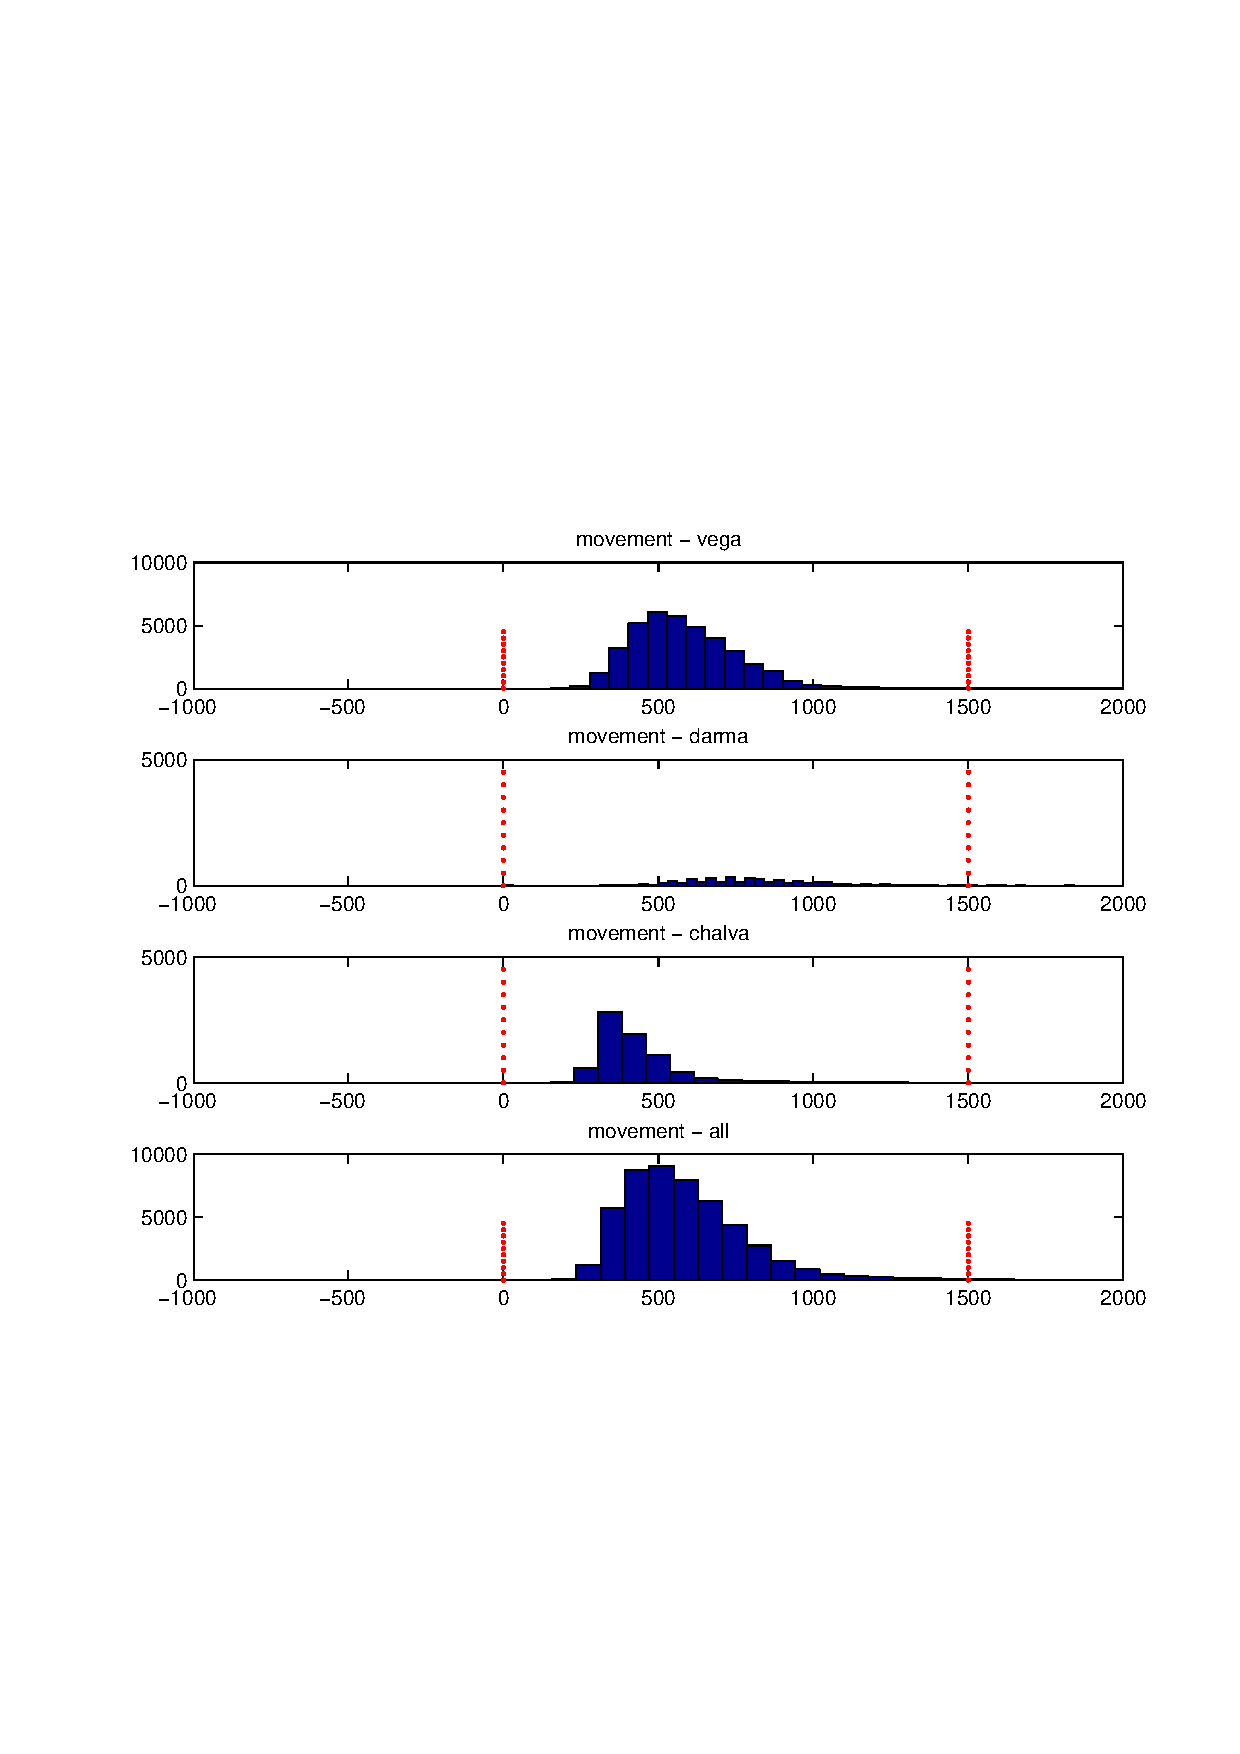
\includegraphics[width=0.3\textwidth]{images/movement.pdf}
    \label{fig:behav:movement}
    }
    \subfigure[Movement Time]{
    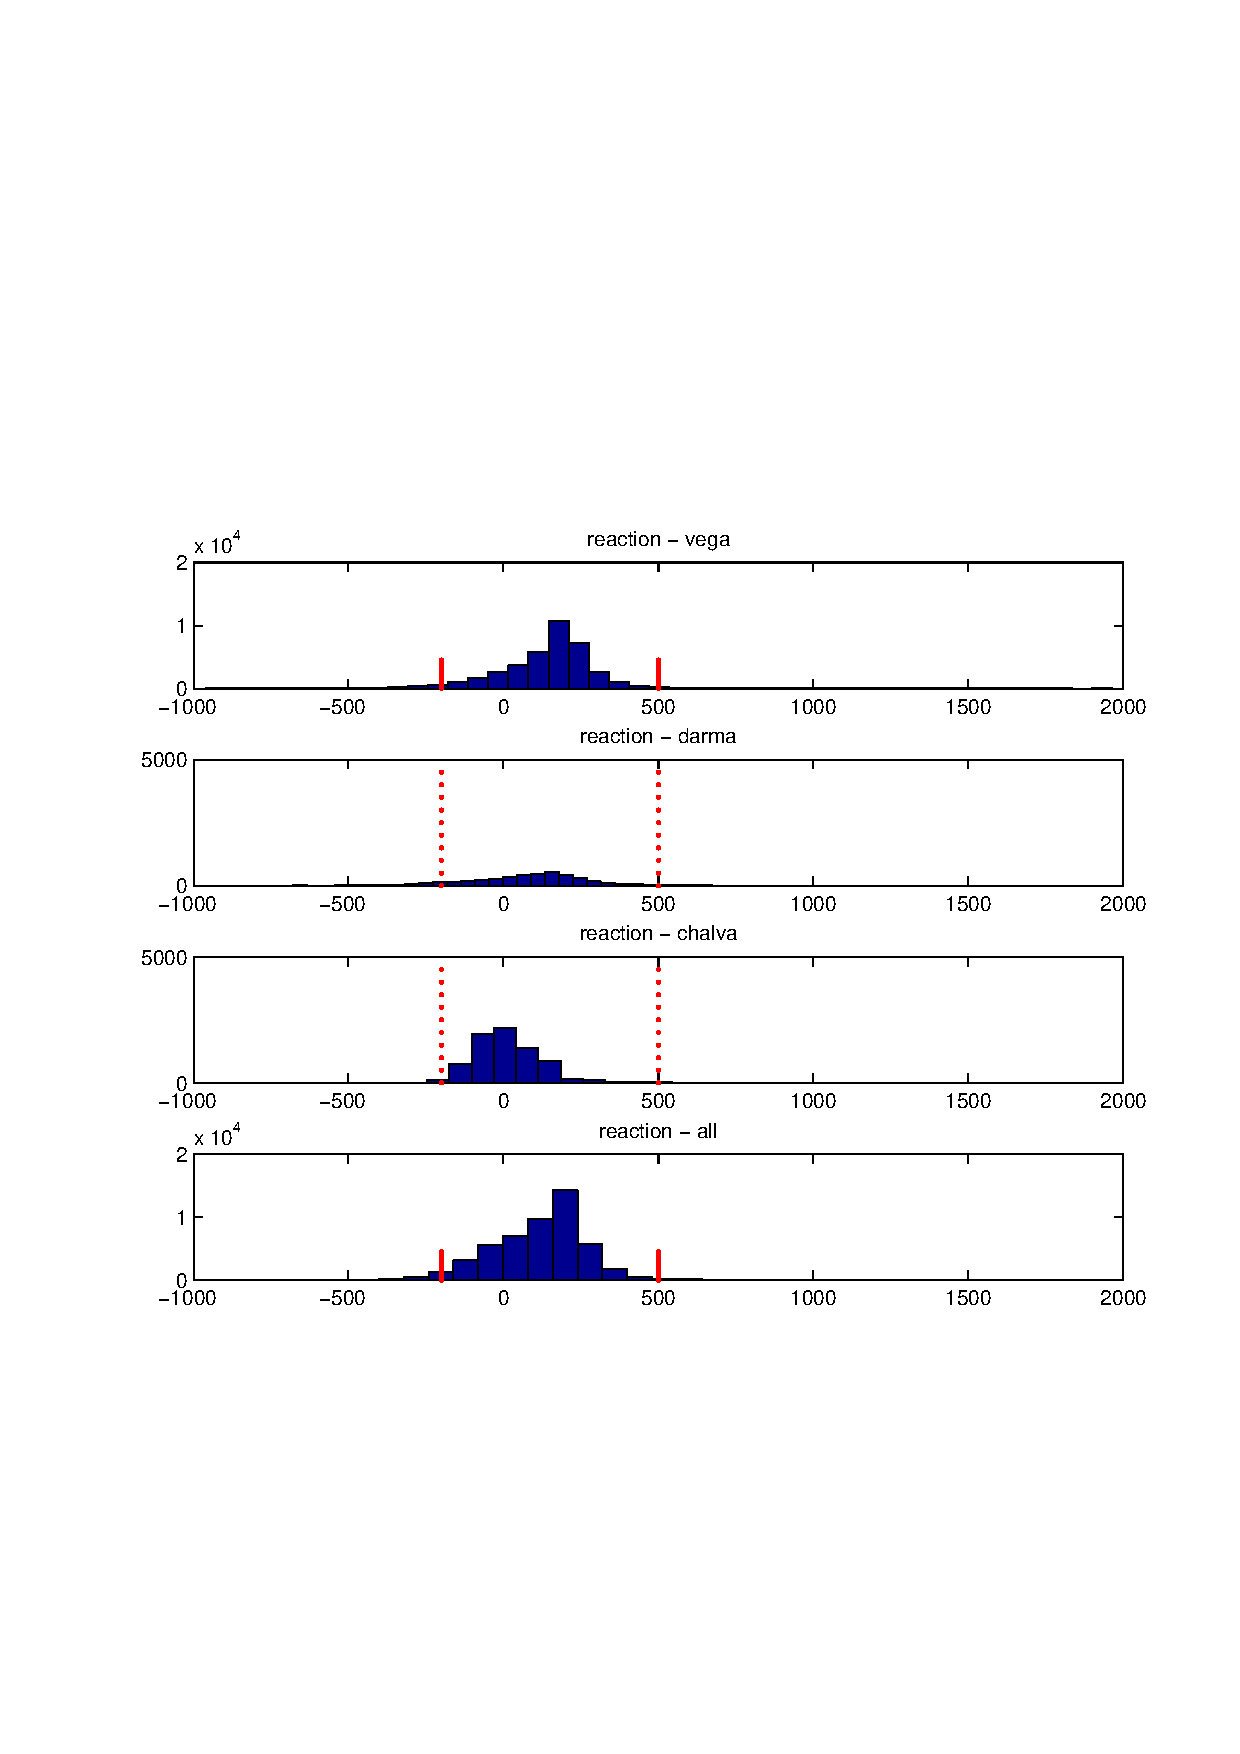
\includegraphics[width=0.3\textwidth]{images/reaction.pdf}
    \label{fig:behav:reaction}
    }
    \subfigure[Angular deviation]{
    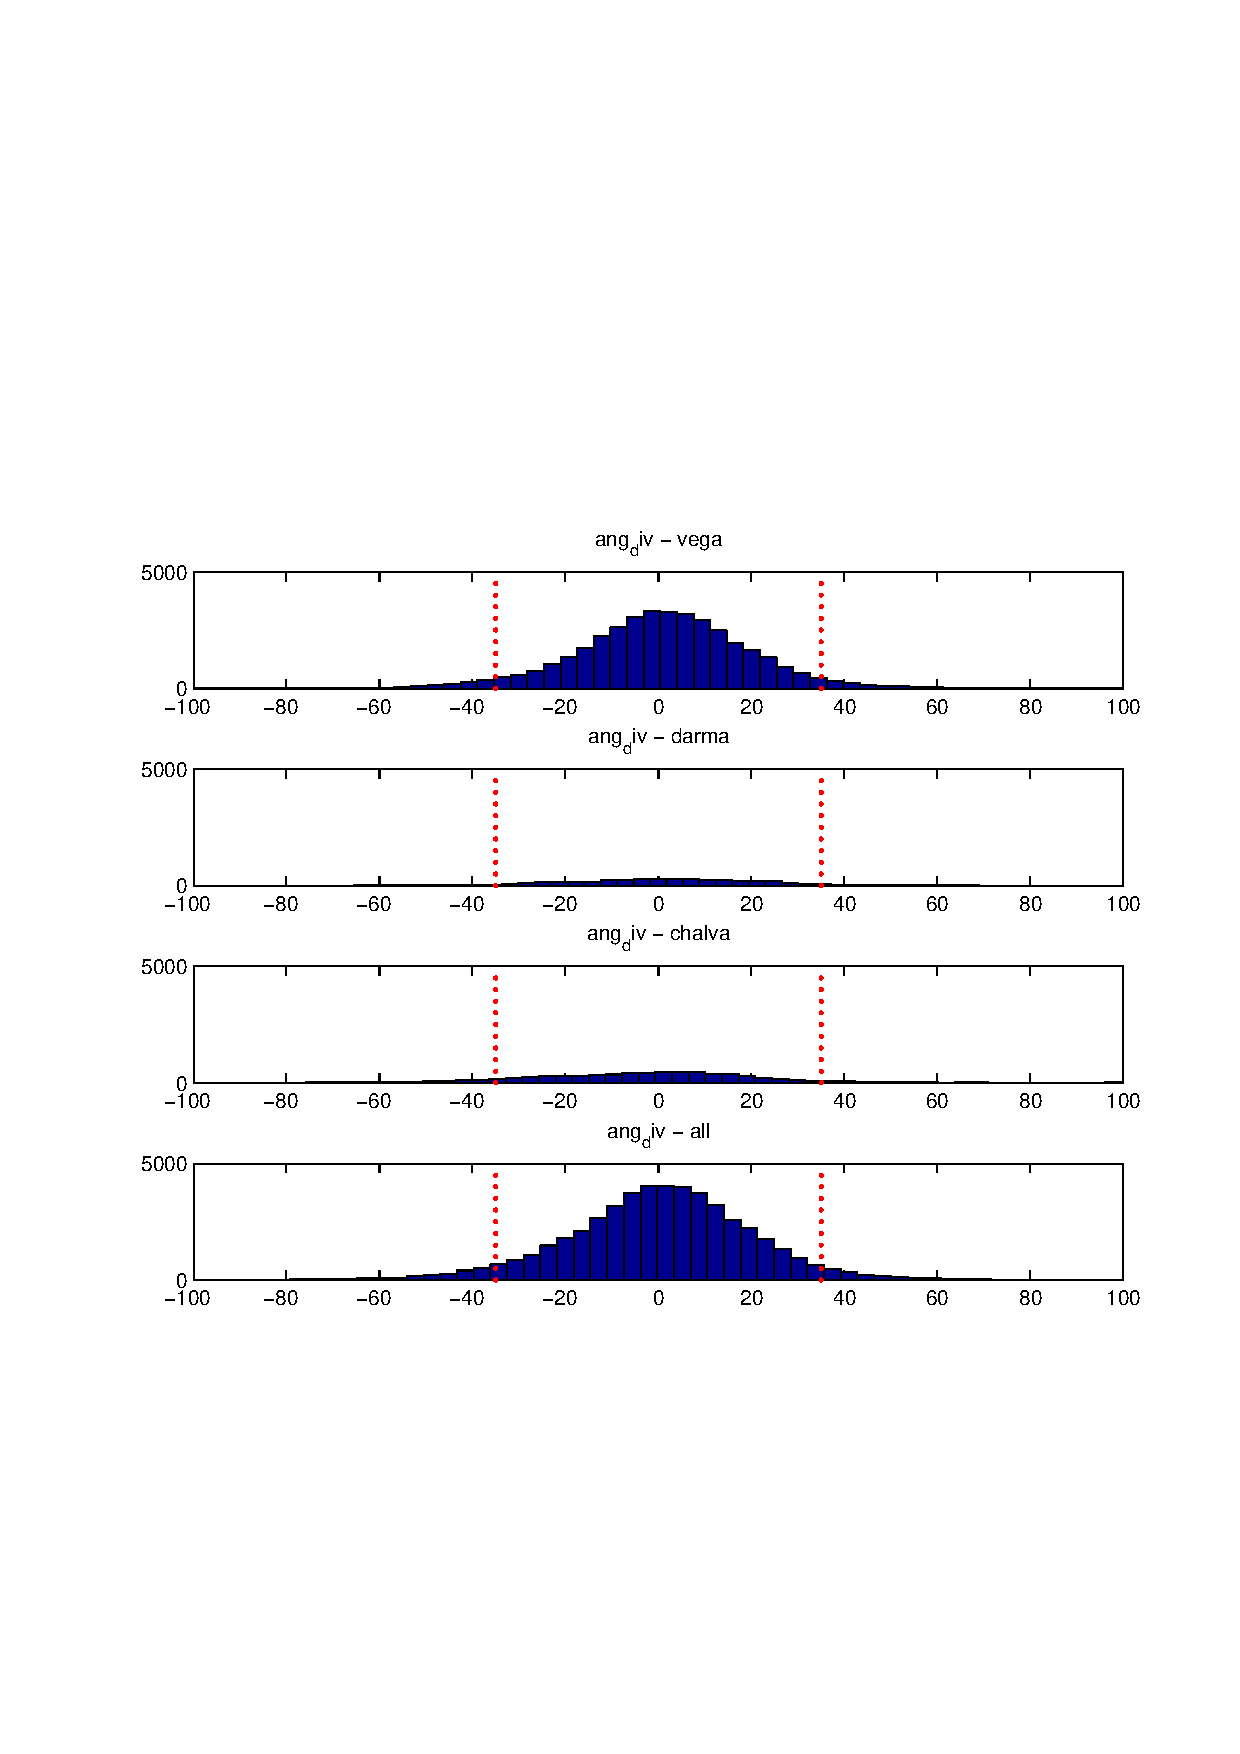
\includegraphics[width=0.3\textwidth]{images/ang_div.pdf}
    \label{fig:behav:ang_div}
    }    
    \caption{Distribution of behavioral criteria which were used for the selection of valid trials. This is done to prevent outliers to influence the further analysis of the data. The selection criteria are chosen to discard only trials where the monkey failed in performing the task correctly.}
    \label{sg:fig:images_behav_crit}
\end{figure}
For all monkeys together there is data from in total 116 sessions available, in which EMG was recorded. Sessions were excluded from further analysis when the data suggested that a session does not represent a typical recording day or that there was something wrong with the data. The criteria for exclusion are defined as:

\begin{description}
    \item[not enough trials] It is data from less then \textbf{50} trials available. This affected only very few sessions as the average number of trials was 292.
    \item[unstable PD] As the preferred direction of a muscle showed to be stable over sessions, sessions where this was not the case were excluded. The criteria for exclusion was that the distance of a sessions PD to the average PD of this channel had to be larger than 2 standard deviations for more than 4 channels.
    \item[rank 1] when the remaining-error of the rank 1 model was already less than 25 \% the session was excluded.
\end{description}
The selection was done by using the pronation position as supination was not available for all sessions and the rank 1 values for the two conditions are also highly correlated (r: 0.77, p << 0.001).


% table of all available data 
\begin{table}[ht]
	\centering
	\begin{tabular}{r|c|c|c}
		\toprule
		                    & vega  & darma & chalva \\
		\toprule
		total (with EMG)    & 91    & 10    & 15\\
		less than 50 trials & 2     & 0     & 0\\
		unstable pds        & 8     & 0     & 1\\
		rank1               & 2     & 0     & 0\\
		\bottomrule
		remaining           & 79    & 10    & 14\\		
		\bottomrule
	\end{tabular}
	\caption{}
	\label{sg:tab:sorting_table_nat}	
\end{table}


% pd stability
\subsection{Preferred directions} % (fold)
\label{sg:sub:preferred_directions}
A plot of the preferred directions over sessions shows that they are stable over sessions and mostly have a significant p value. For all monkeys most of the channels have high significance values and low circular standard deviation. This allows to compute the circular mean. Less significance or higher variance in a channel does not necessarily mean that the recording was noisy. It can just mean that the muscle is not so much tuned to a special direction or that the tuning is dependent on the posture. This is shown e.g. for channel 9 of subject V \subref{fig:pd_bar:v} as it shows good stability for one hand-position but not for the other one. Therefore small significance does not mean noisy channel but only that a muscle is more untuned. In \rref{sg:fig:pd_barplots} it is visible that the selection of only significant PDs does not influence the outcome of the \emph{cstd} very much.

% preferred direction barplots
\begin{figure}[ht]
    \centering
    \subfigure[subject C]{
    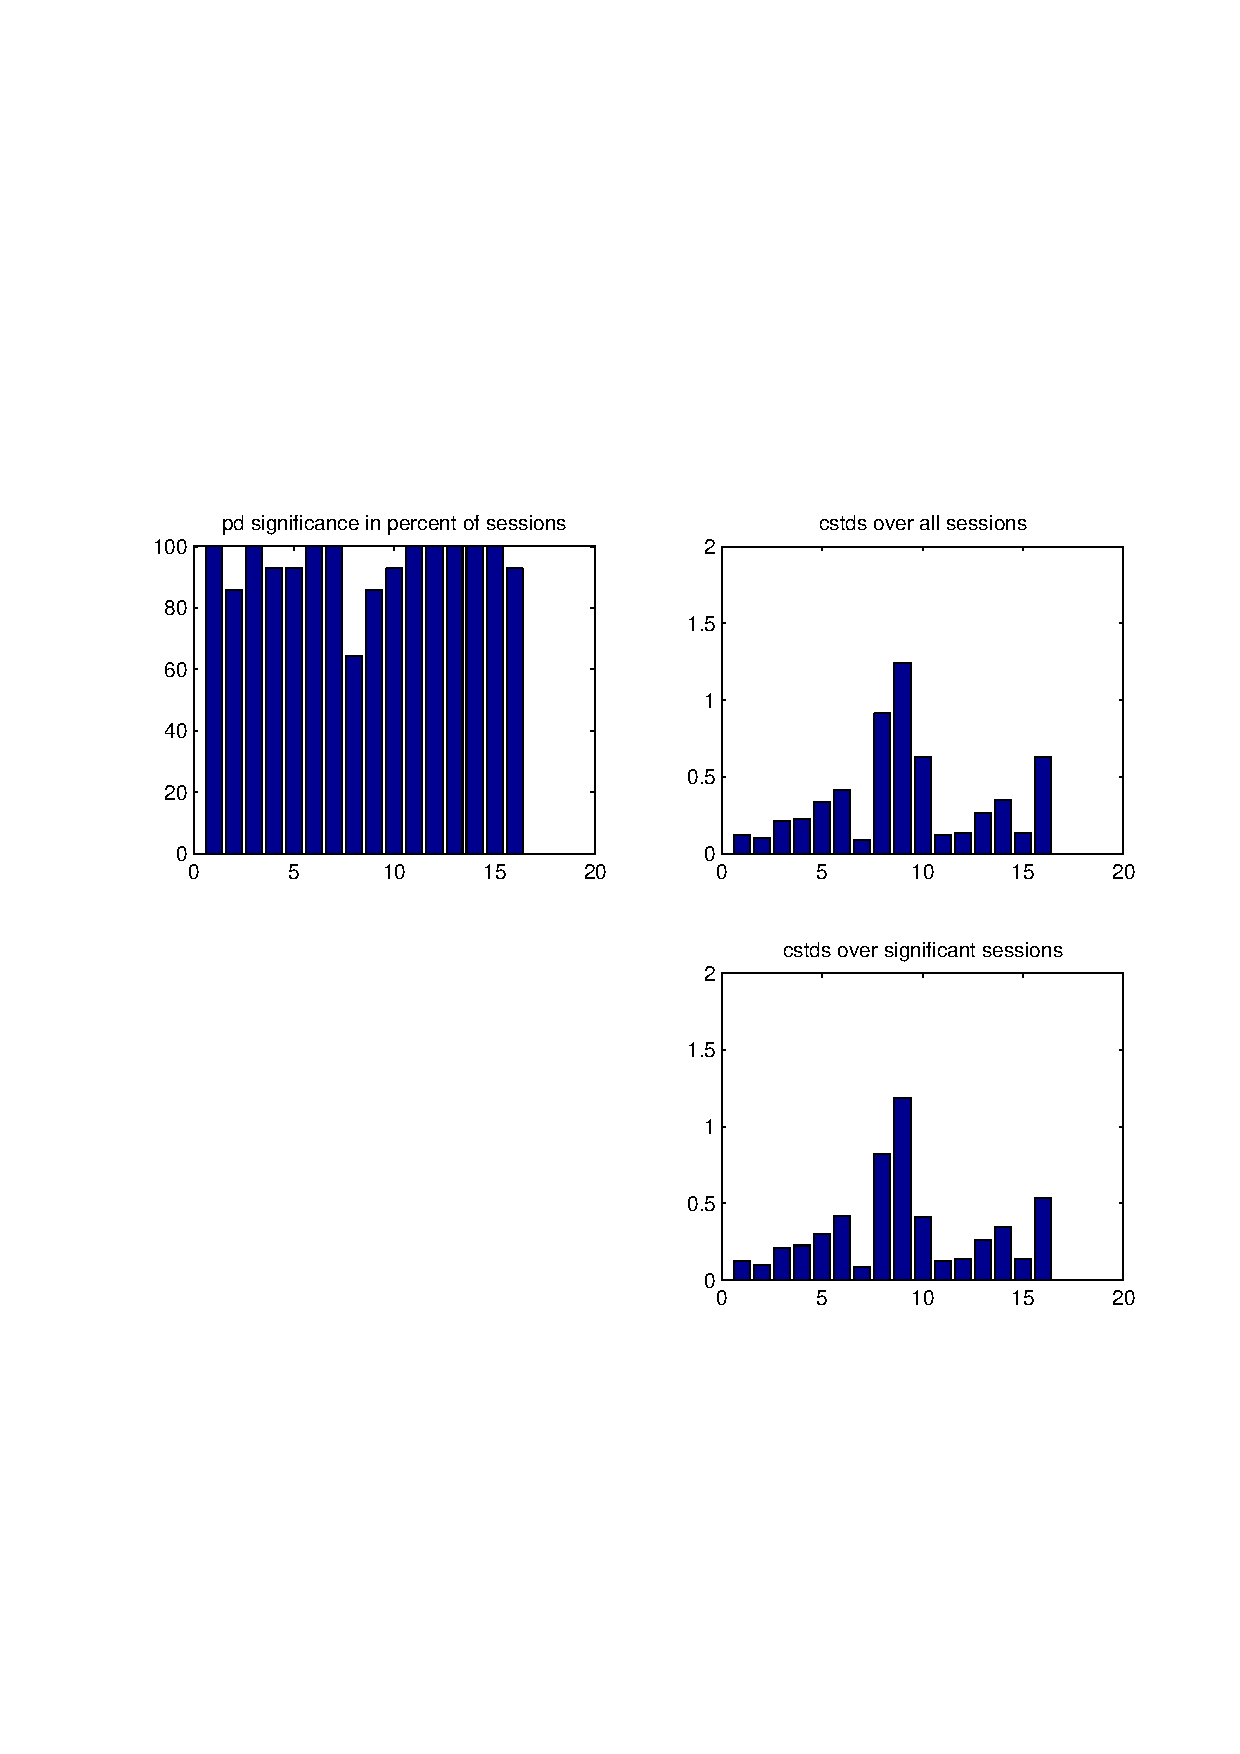
\includegraphics[width=0.3\textwidth]{images/pd_consist_bars_chalva.pdf}
    \label{fig:pd_bar:c}
    }
    \subfigure[subject D]{
    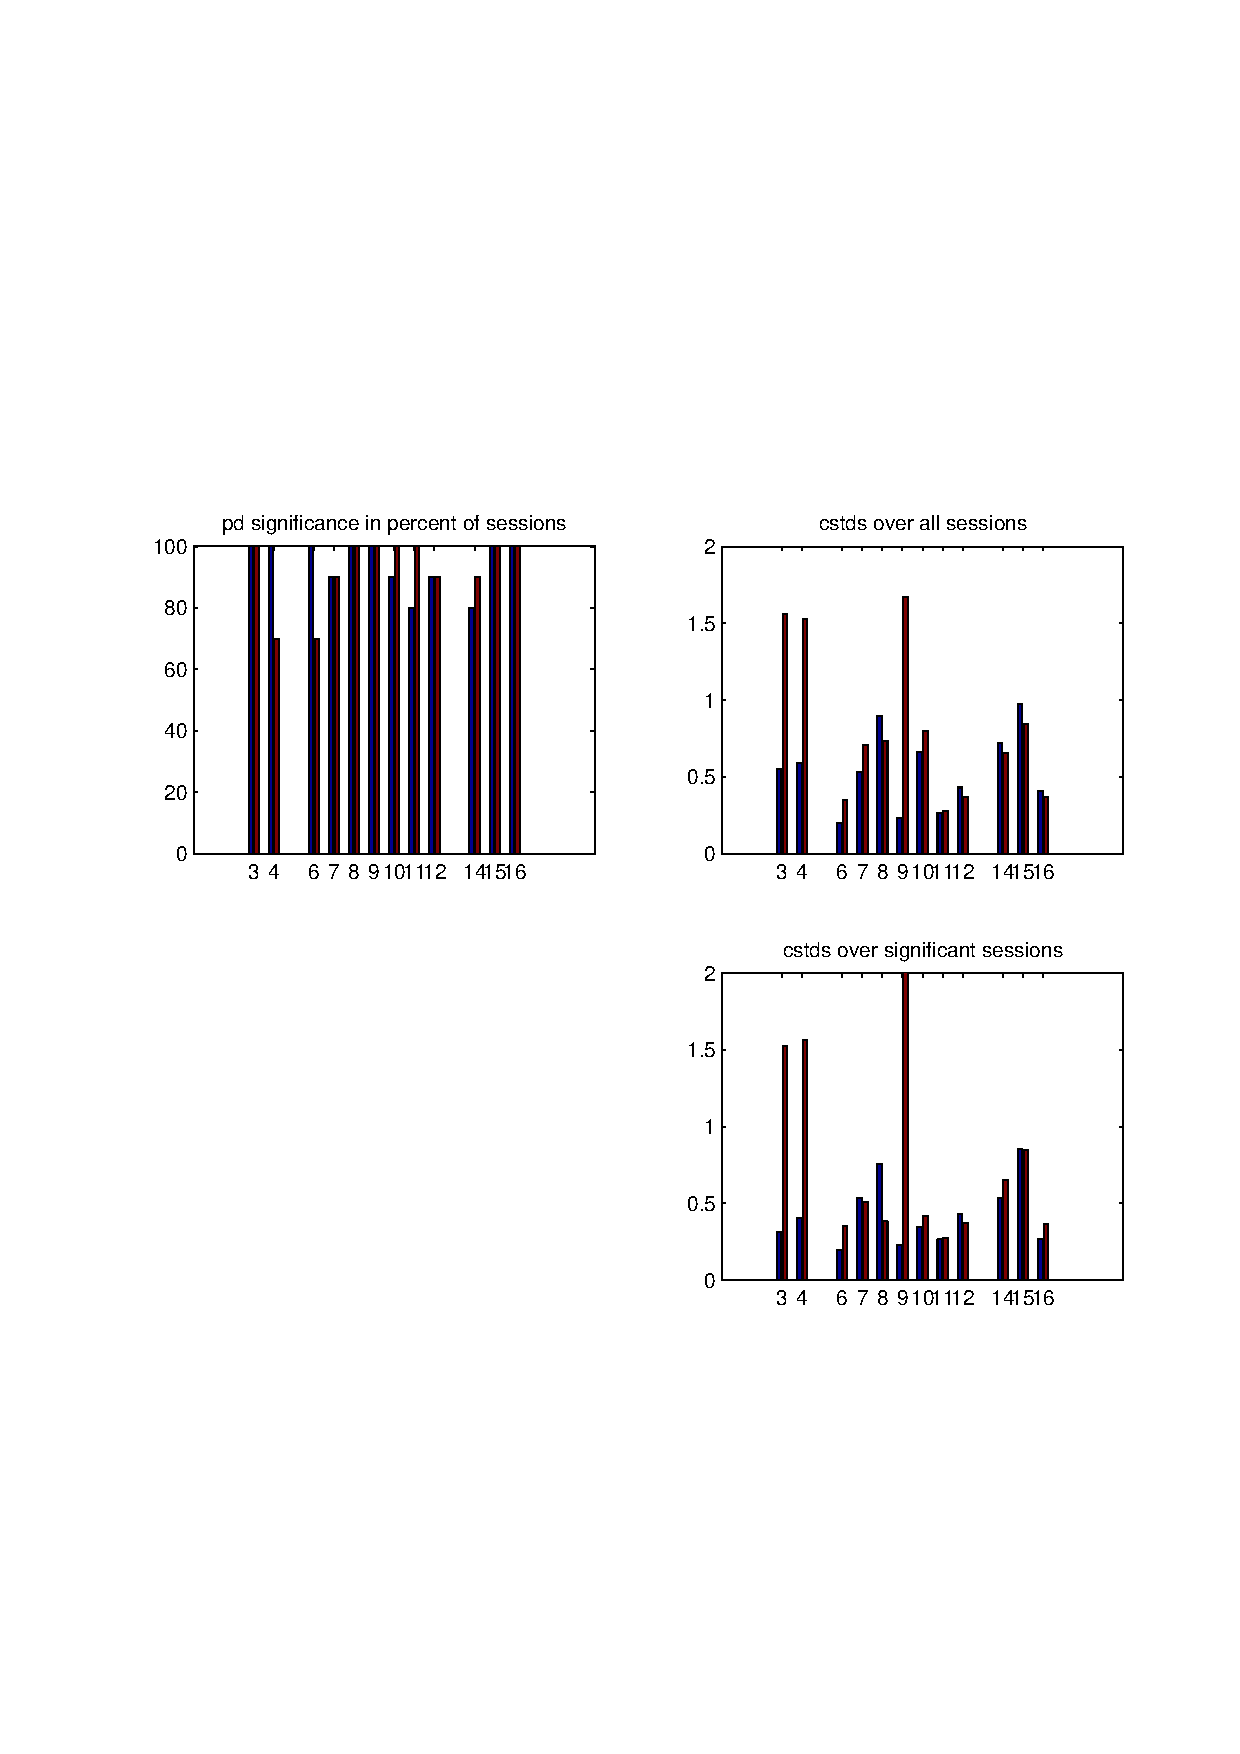
\includegraphics[width=0.3\textwidth]{images/pd_consist_bars_darma.pdf}
    \label{fig:pd_bar:d}
    }
    \subfigure[subject V]{
    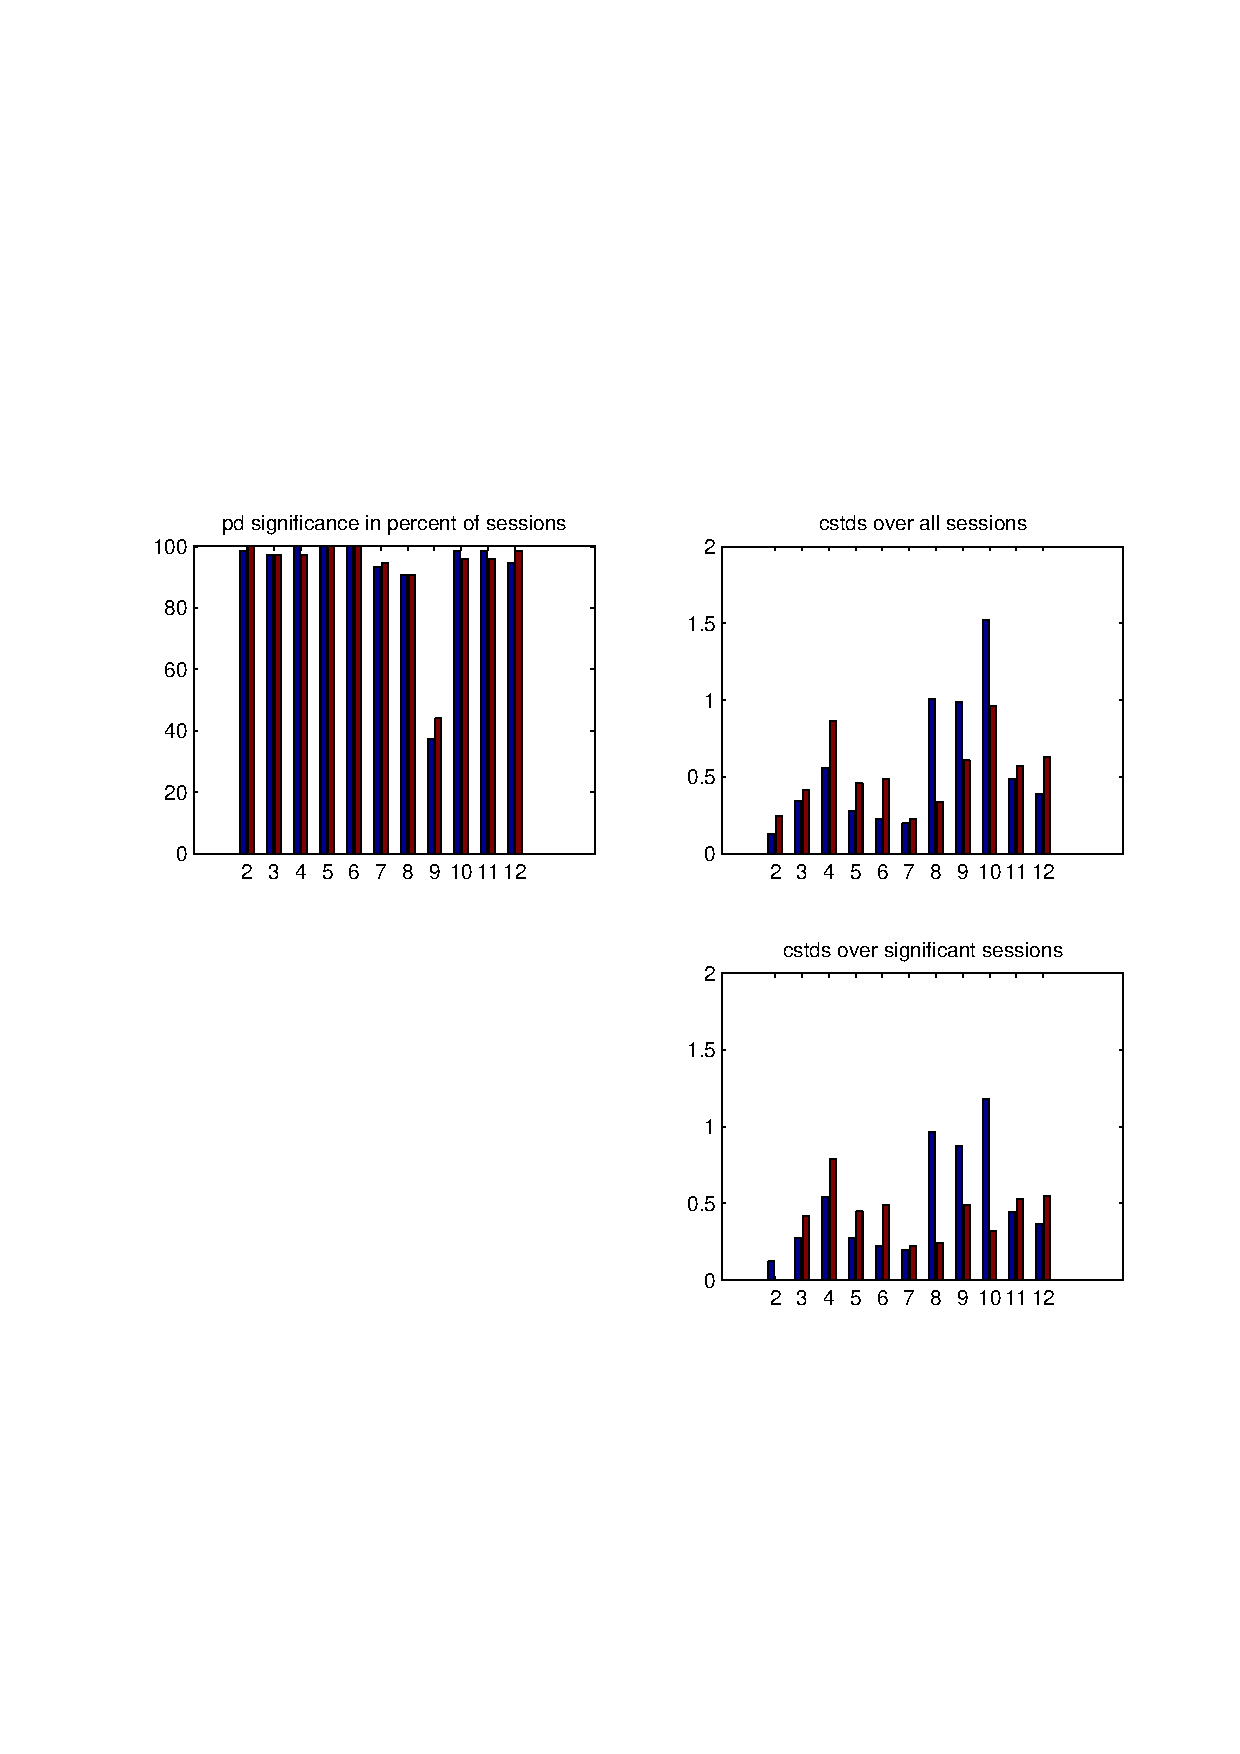
\includegraphics[width=0.3\textwidth]{images/pd_consist_bars_vega.pdf}
    \label{fig:pd_bar:v}
    }    
    \caption{For all subjects in most of the channels the preferred directions are are significantly tuned. In the plot it is also visible that the PDs were stable over sessions which is expressed in low values of the standard deviation. But also when they are not significantly tuned, it does not mean that the recording was noisy but rather that a certain muscle is not so much tuned for a certain direction. How much a muscle is tuned for a certain direction can also depend on the posture. The significance of a preferred direction does not have large influence on the \emph{cstd}.}
    \label{sg:fig:pd_barplots}
\end{figure}

% preferred direction featherplots
\begin{figure}[ht]
    \centering
    \subfigure[subject C]{
    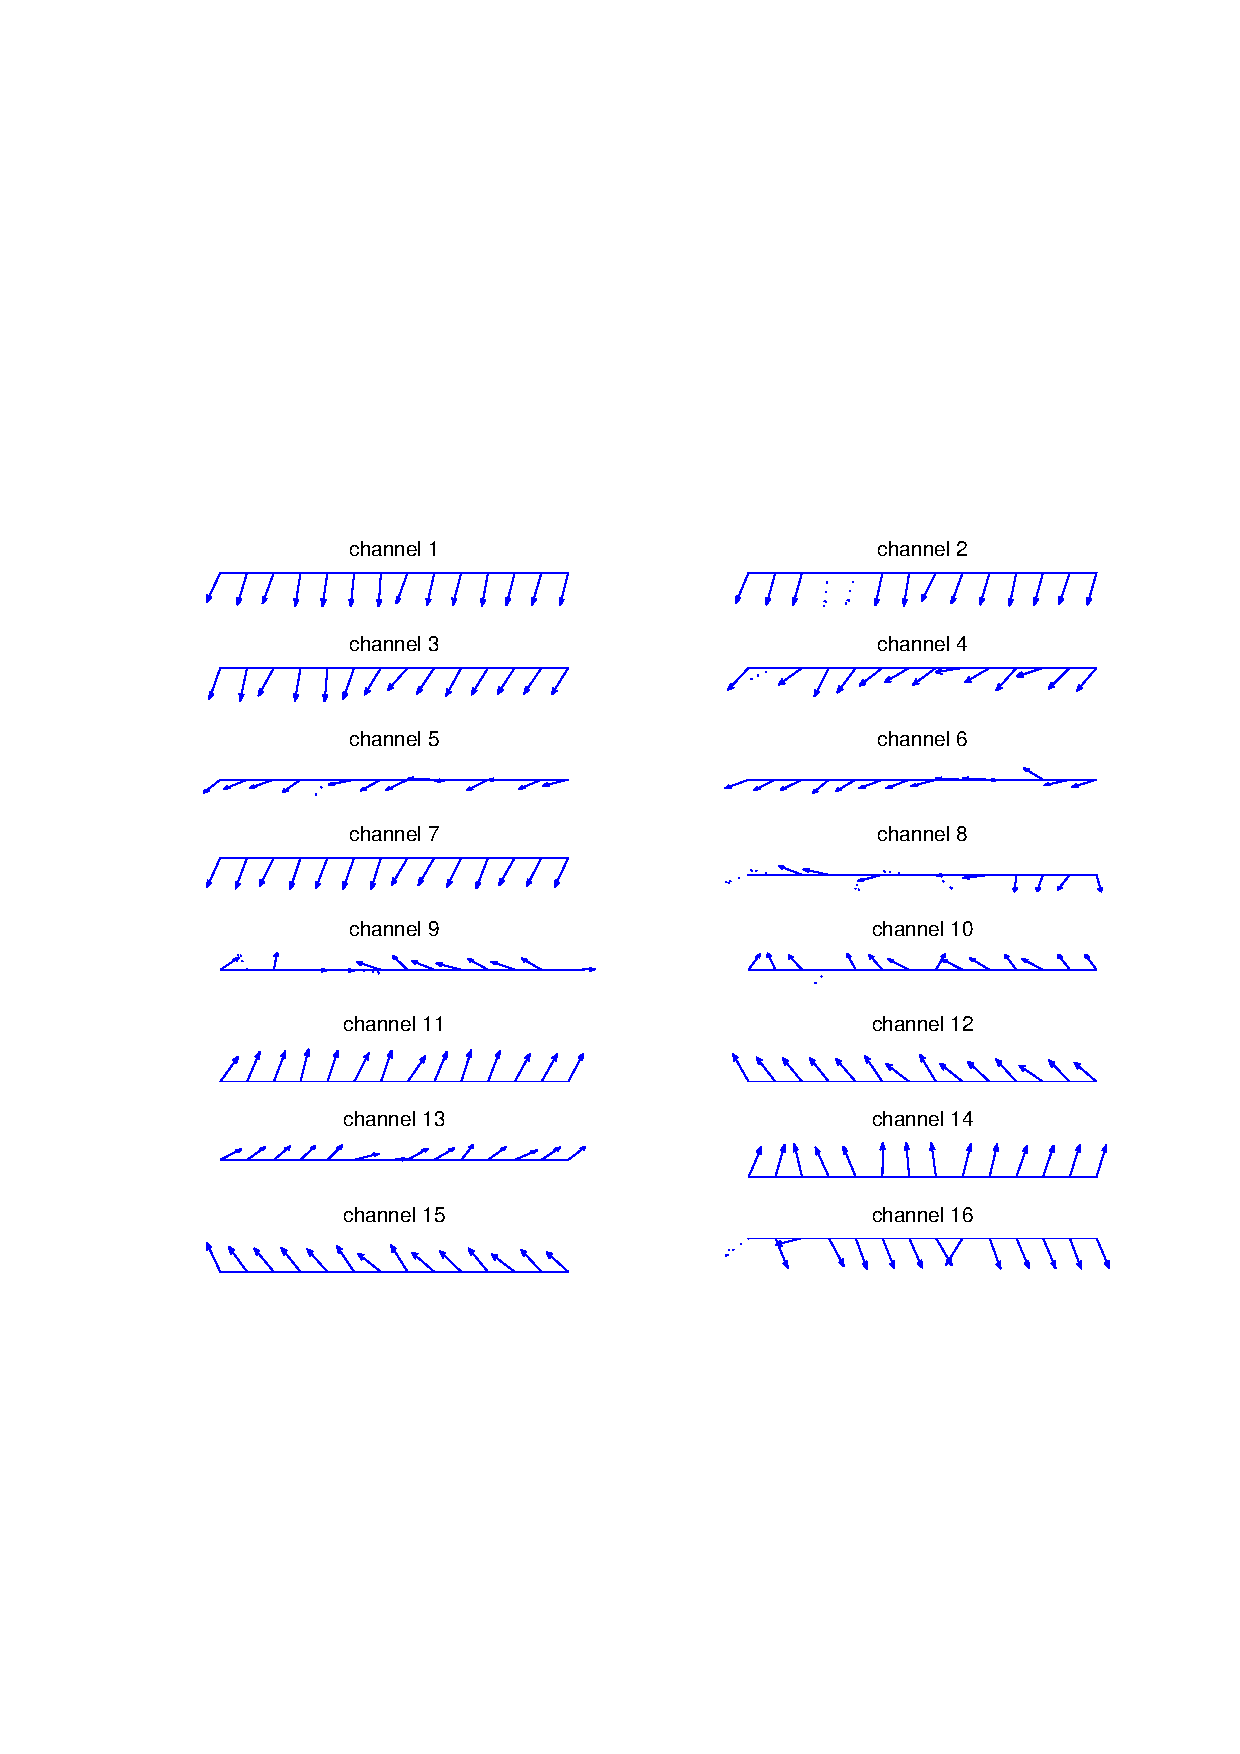
\includegraphics[width=0.3\textwidth]{images/pd_consist_feather_chalva.pdf}
    \label{fig:pd_feather:c}
    }
    \subfigure[subject D]{
    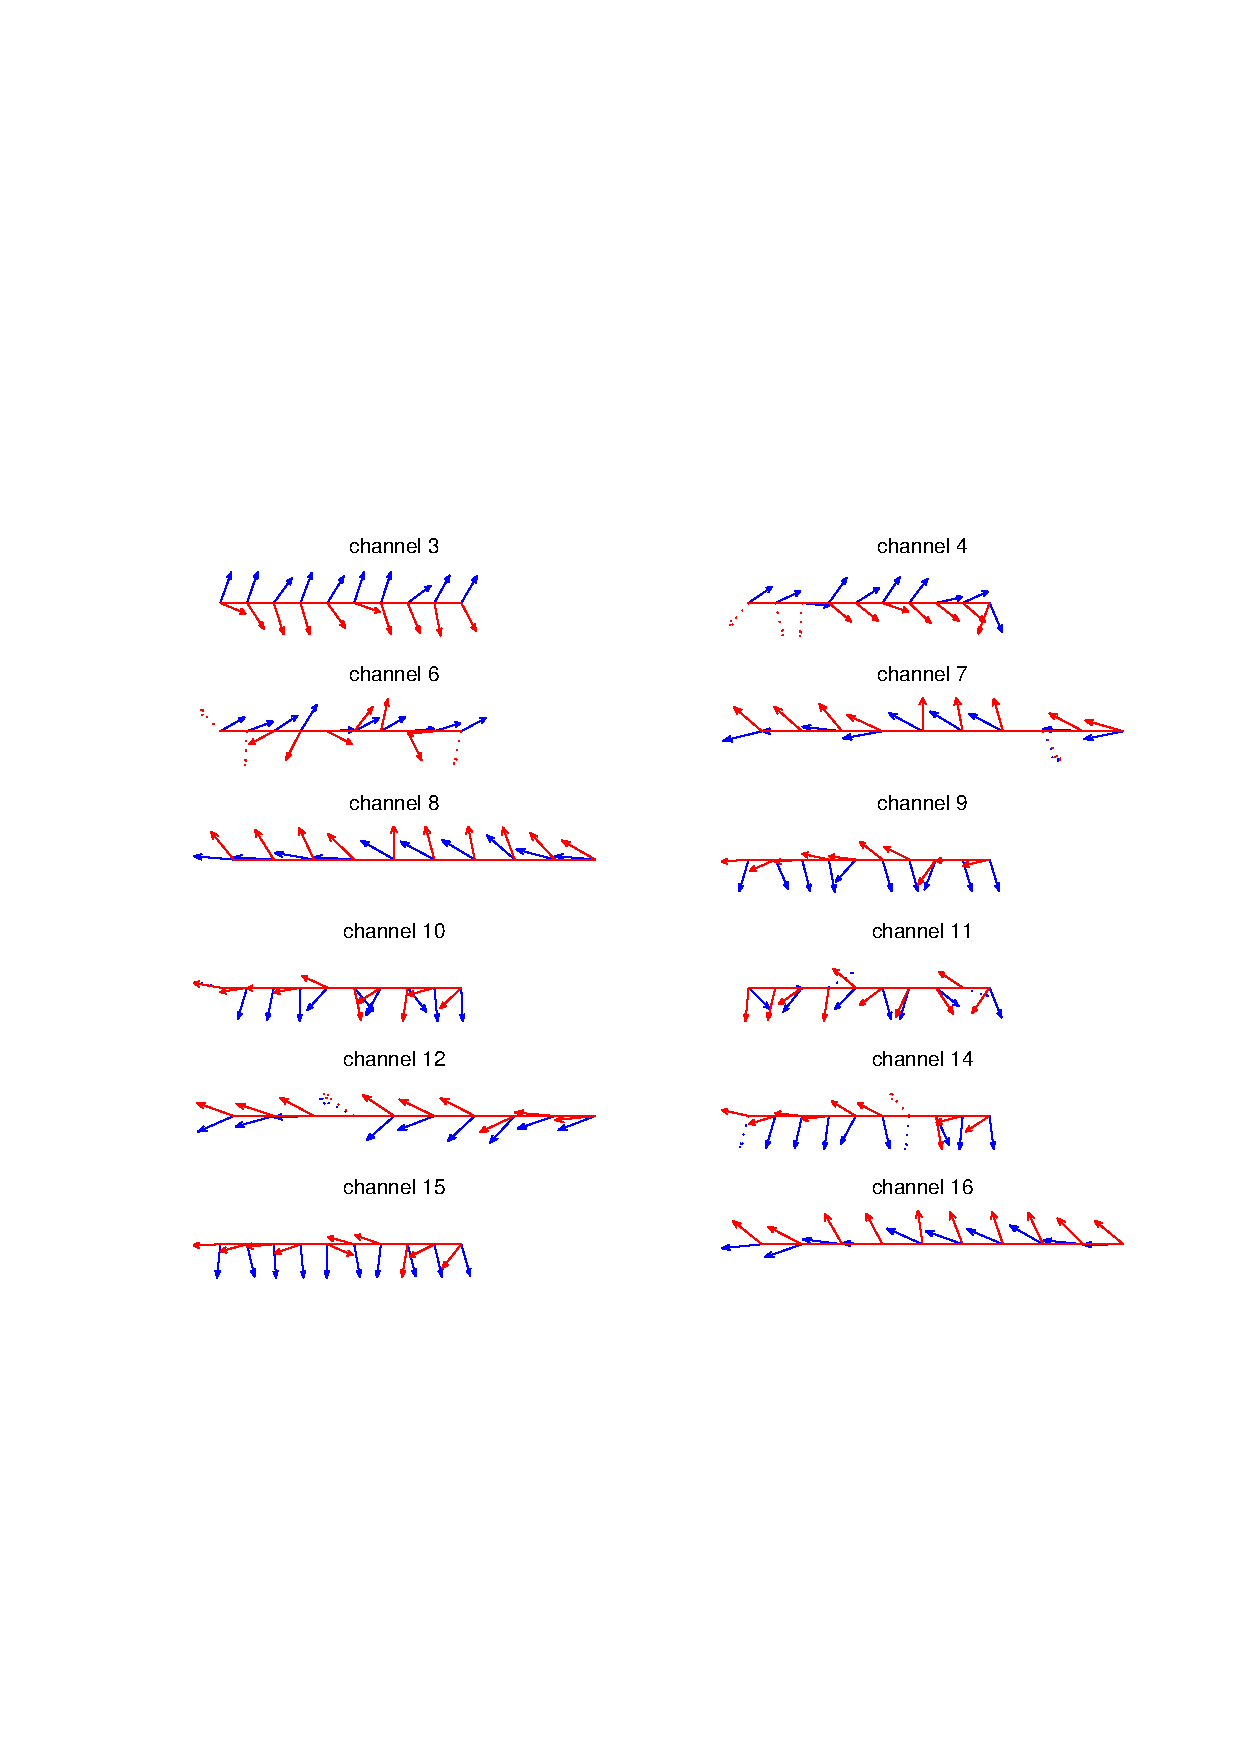
\includegraphics[width=0.3\textwidth]{images/pd_consist_feather_darma.pdf}
    \label{fig:pd_feather:d}
    }
    \subfigure[subject V]{
    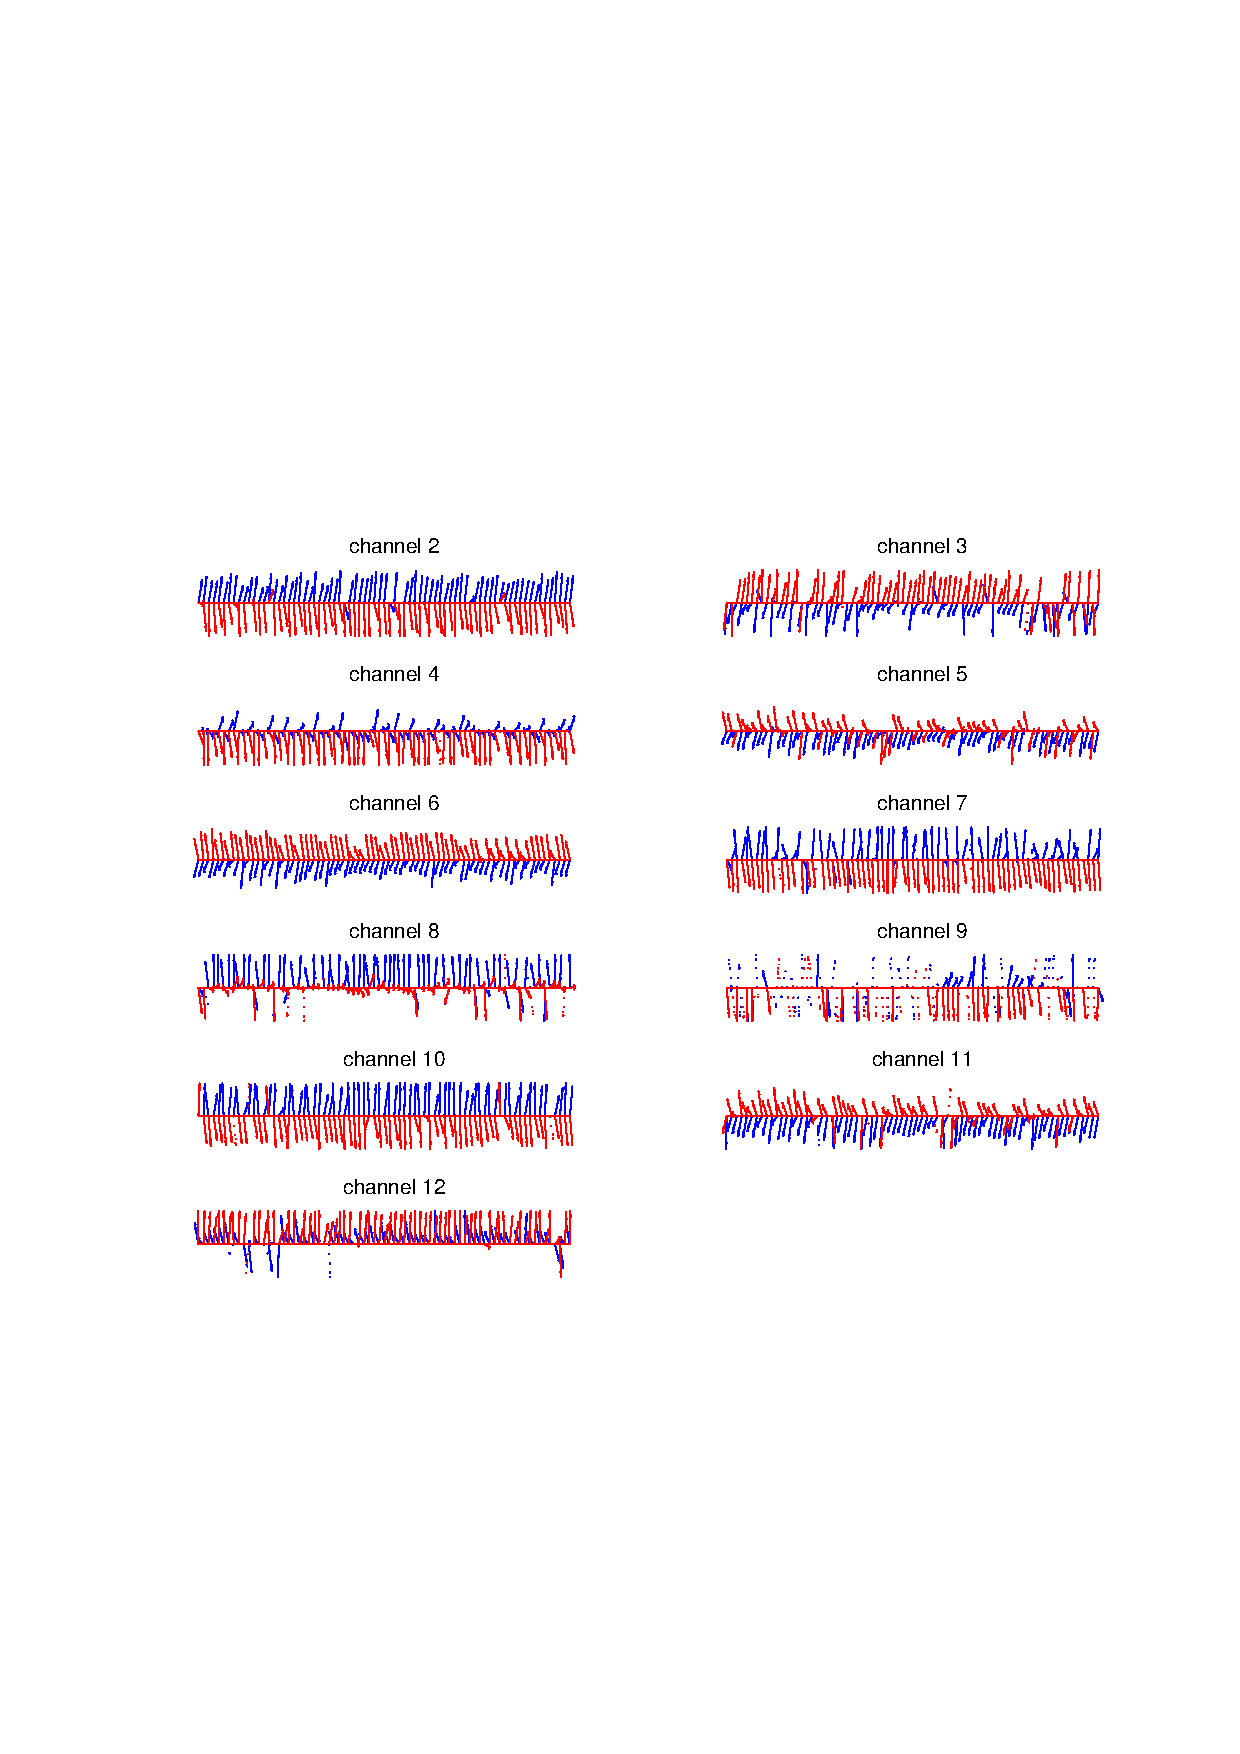
\includegraphics[width=0.3\textwidth]{images/pd_consist_feather_vega.pdf}
    \label{fig:pd_feather:v}
    }    
    \caption{This plot shows the PDs of channels in a more intuitive feather plot. Each arrow corresponds to the preferred direction of a sessions which makes it easy to see consistency over sessions (all arrows would point in the same direction). Preferred directions which are not tuned significantly are plotted with a dashed line. Please not that the PD is not necessarily and outlier when a muscle is not significantly tuned.}
    \label{sg:fig:pd_featherplots}
\end{figure}
\clearpage
% subsection preferred_directions (end)


After the computation of evoked muscle-activation, the data was in form of a $\mathrm{trials} \times \mathrm{channels}$ matrix for each session and hand position. The whole subsequent analysis was always performed in parallel for separated hand positions and also for a $(\mathrm{supination trials} + \mathrm{pronation trials}) \times \mathrm{channels}$ 2-D matrix, containing the data for both hand positions. First the MF-algorithms were applied to the matrices containing pronation-position trying to reduce the dimensionality of the data to only one synergy (rank 1 model order). This was done in order to sort out sessions were EMG signals across channels are highly correlated. The PCAICA-algorithm led to generally smaller error values, but they were highly correlated with the remaining error values of the NMF-algorithm (r: 0.85, p << 0.001). NMF was, due to its biologically plausible assumptions, preferred in the further analysis and therefore also chosen for selection of sessions. 

% rank 1 figure
\begin{figure}[ht]
	\centering
		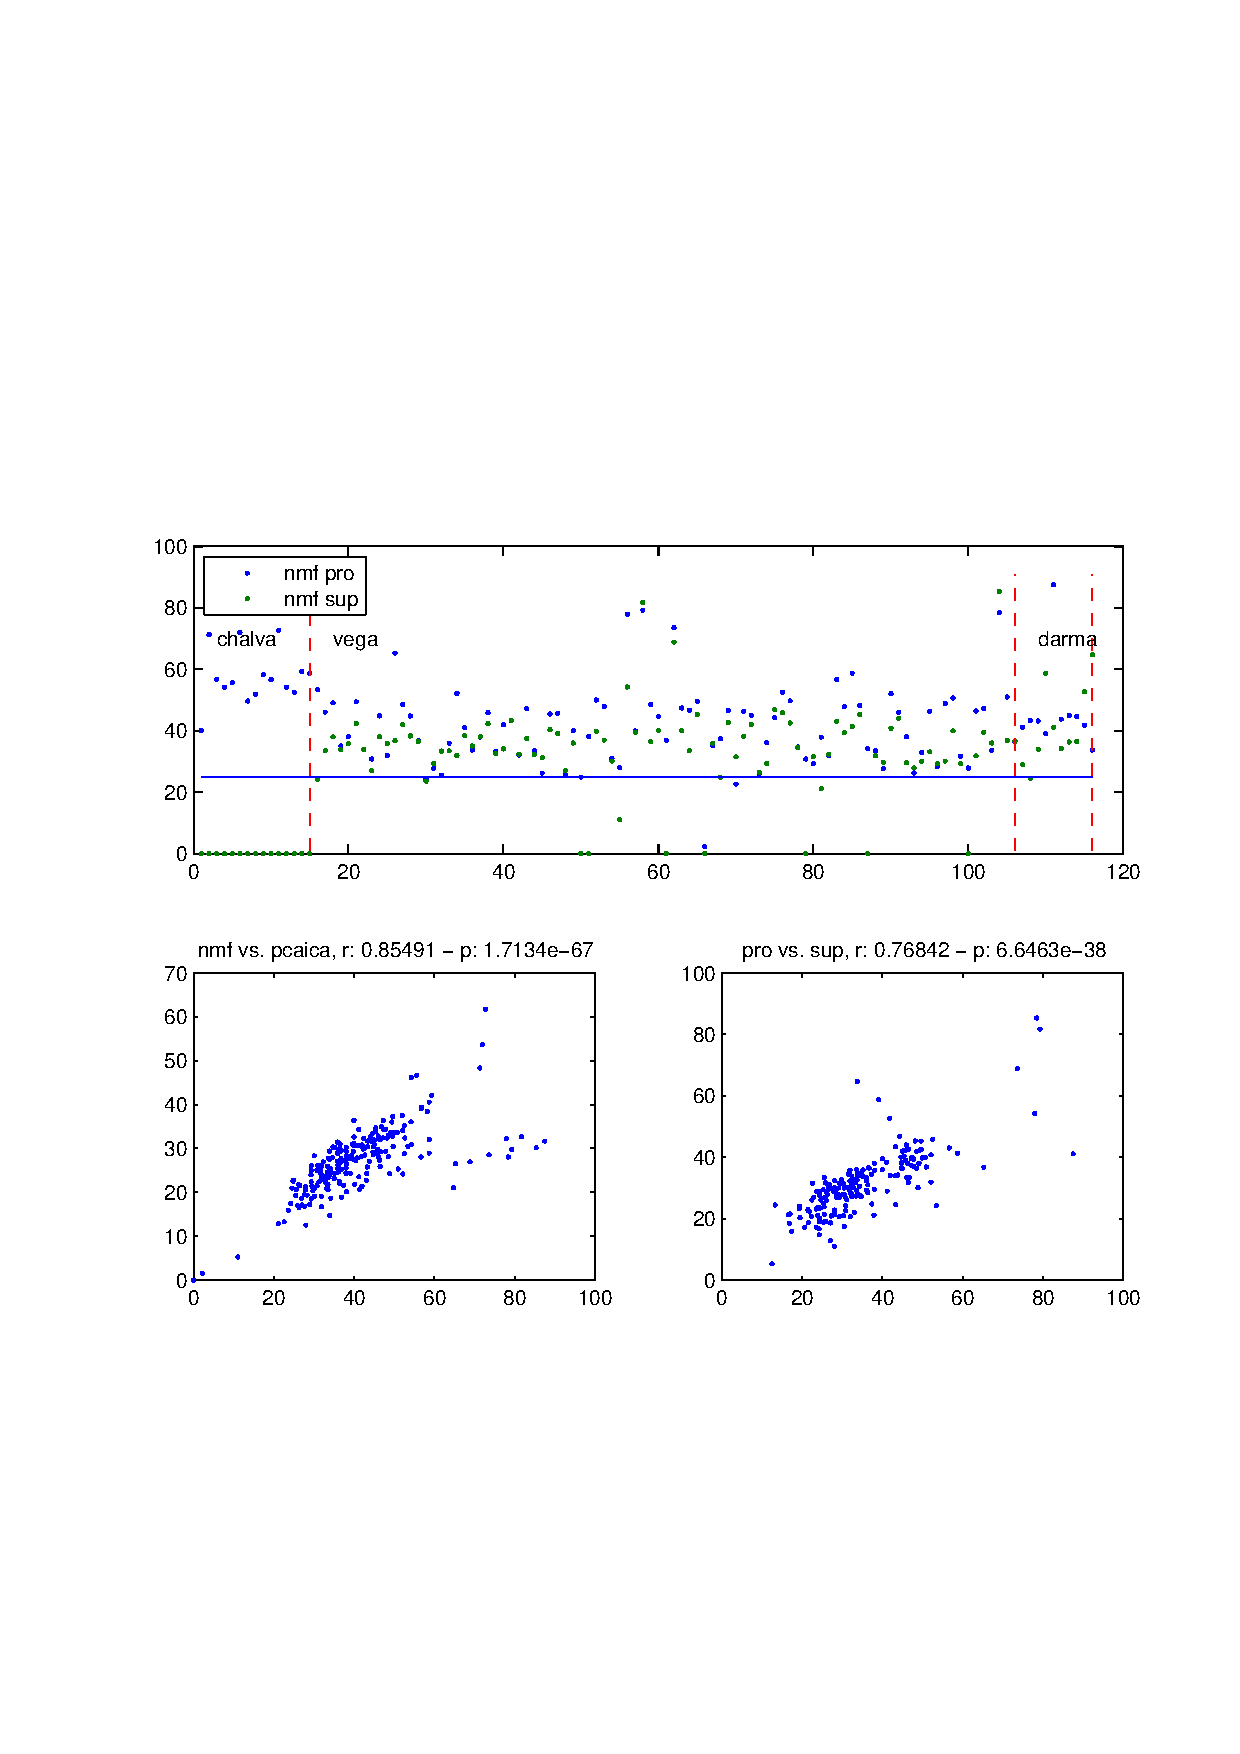
\includegraphics[width=0.7\textwidth]{images/rank1.pdf}
	\caption{
Error values for NMF in pronation and supination when data was reduced to a 1 dimensional model. Sessions with an NMF remaining error higher than 25 \% were chosen for further analysis.
	}
	\label{sg:fig:images_rank1}
\end{figure}


% synergy computation for separated sessions
The NMF remaining error plot suggests, that the data for each session can be reduced to 3 dimensions while still explaining 85 \% of the variance \rref{sg:fig:images_all_resid_non}. It also shows that this is due to the structure of the data as random data with same statistical properties leads to higher error values. Examination of PCAICA error values led to the same results but is not shown here because of the strong correlation between the two measurements in the rank 1 analyses~\rref{sg:fig:images_rank1}.
% all resid nonevoked figure
\begin{figure}[ht]
	\centering
		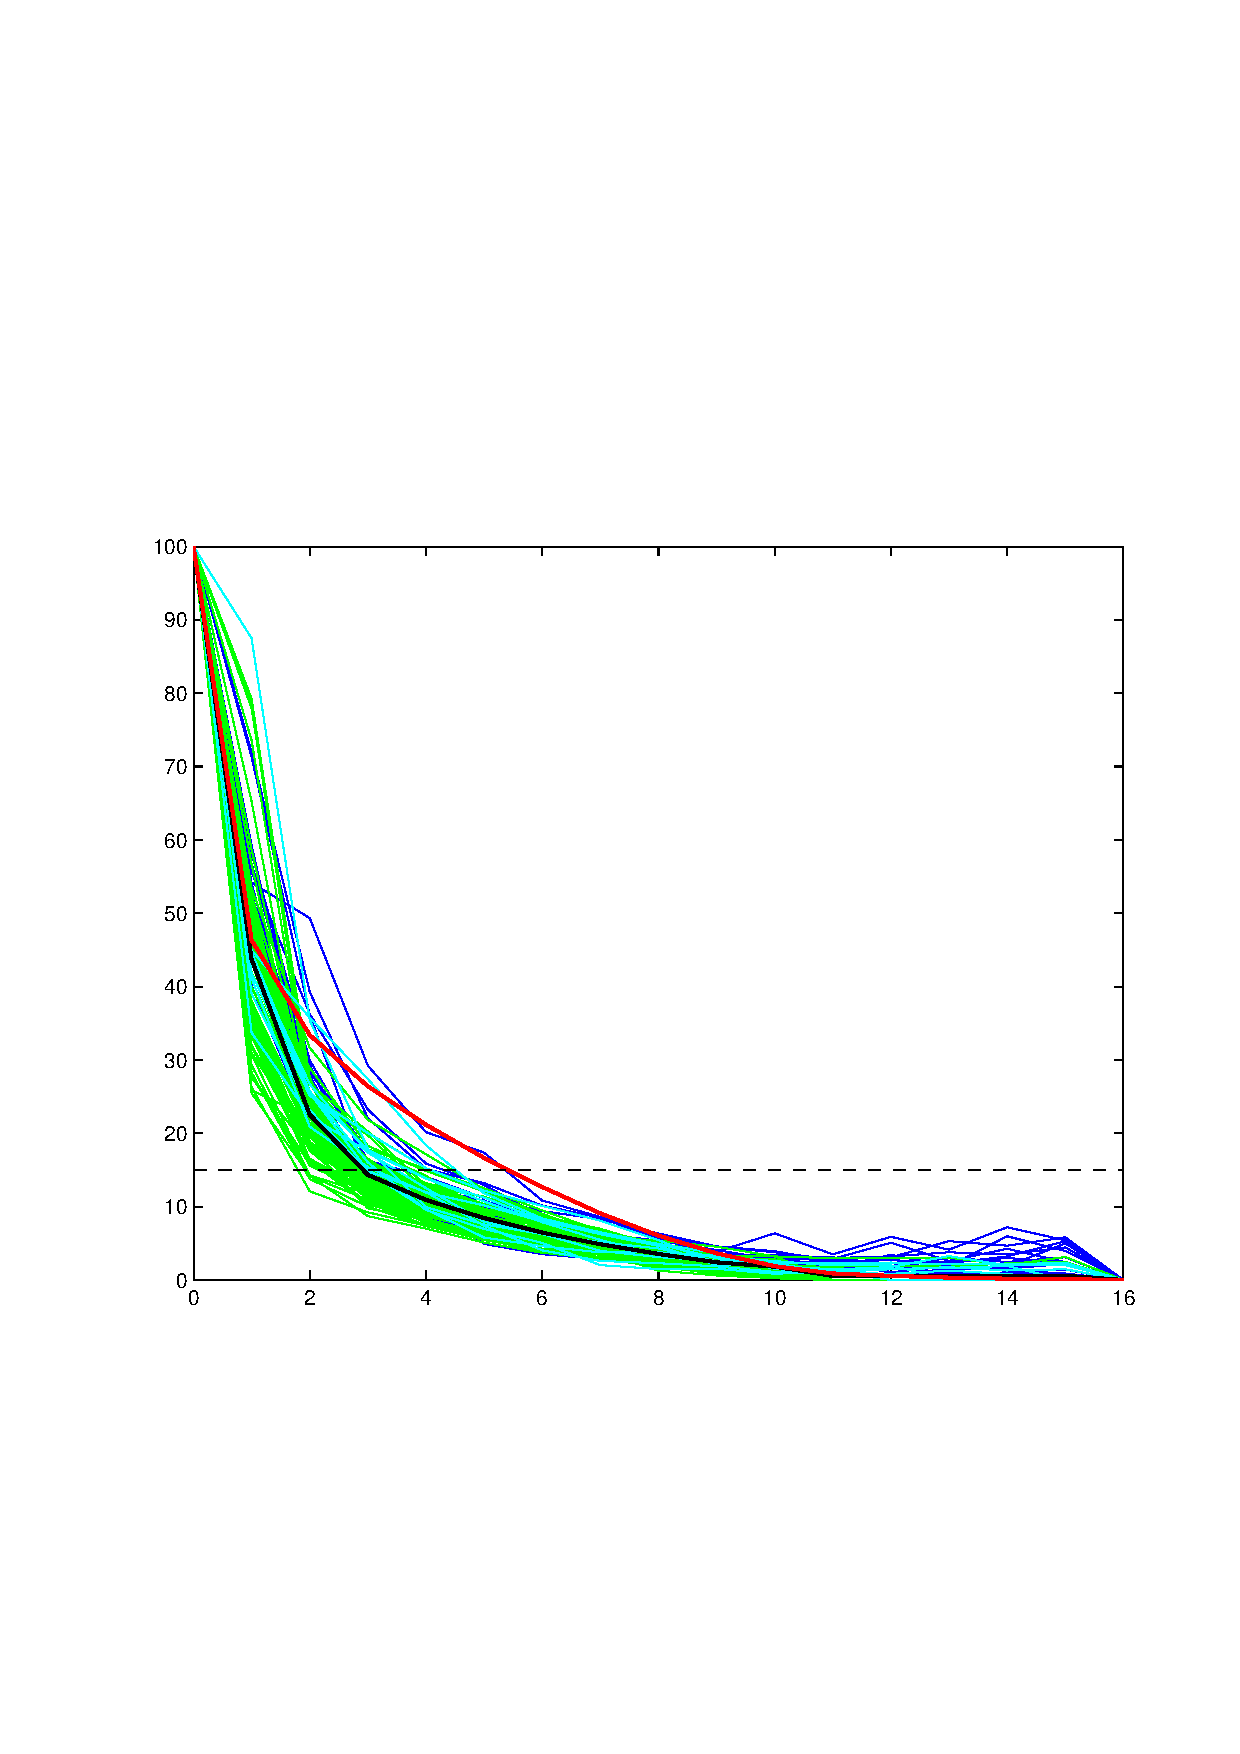
\includegraphics[width=0.9\textwidth]{images/resid_test.pdf}
	\caption
	{
	remaining error for data from pronation hand-position has 15 \% remaining error if reduced to a 3 dimensional model. Randomized data with same statistical properties (shuffled data) shows much higher error values.
	}
	\label{sg:fig:images_all_resid_non}
\end{figure}

To assess the stability of the synergies over sessions, all synergies extracted from single sessions were as in the method to compare NMF stability~\rref{sg:fig:images_nmf_expl_stab3} pooled in one data set and sorted according to a k-means clustering with 3 prototypes. The distribution of group size does not exhibit perfect categorization (STD 0) as in the stability analyses but still shows clear clustering and therefore stable muscle synergies over sessions~\rref{sg:fig:images_syn_consist_sessions_std}. The prototypes of the k-means clustering are the average synergies steadily found over all sessions. This analysis was done for the pronation hand-position as this was available for all monkeys


% nmf stability over sessions (cluster std)
\begin{figure}[ht]
    \centering
    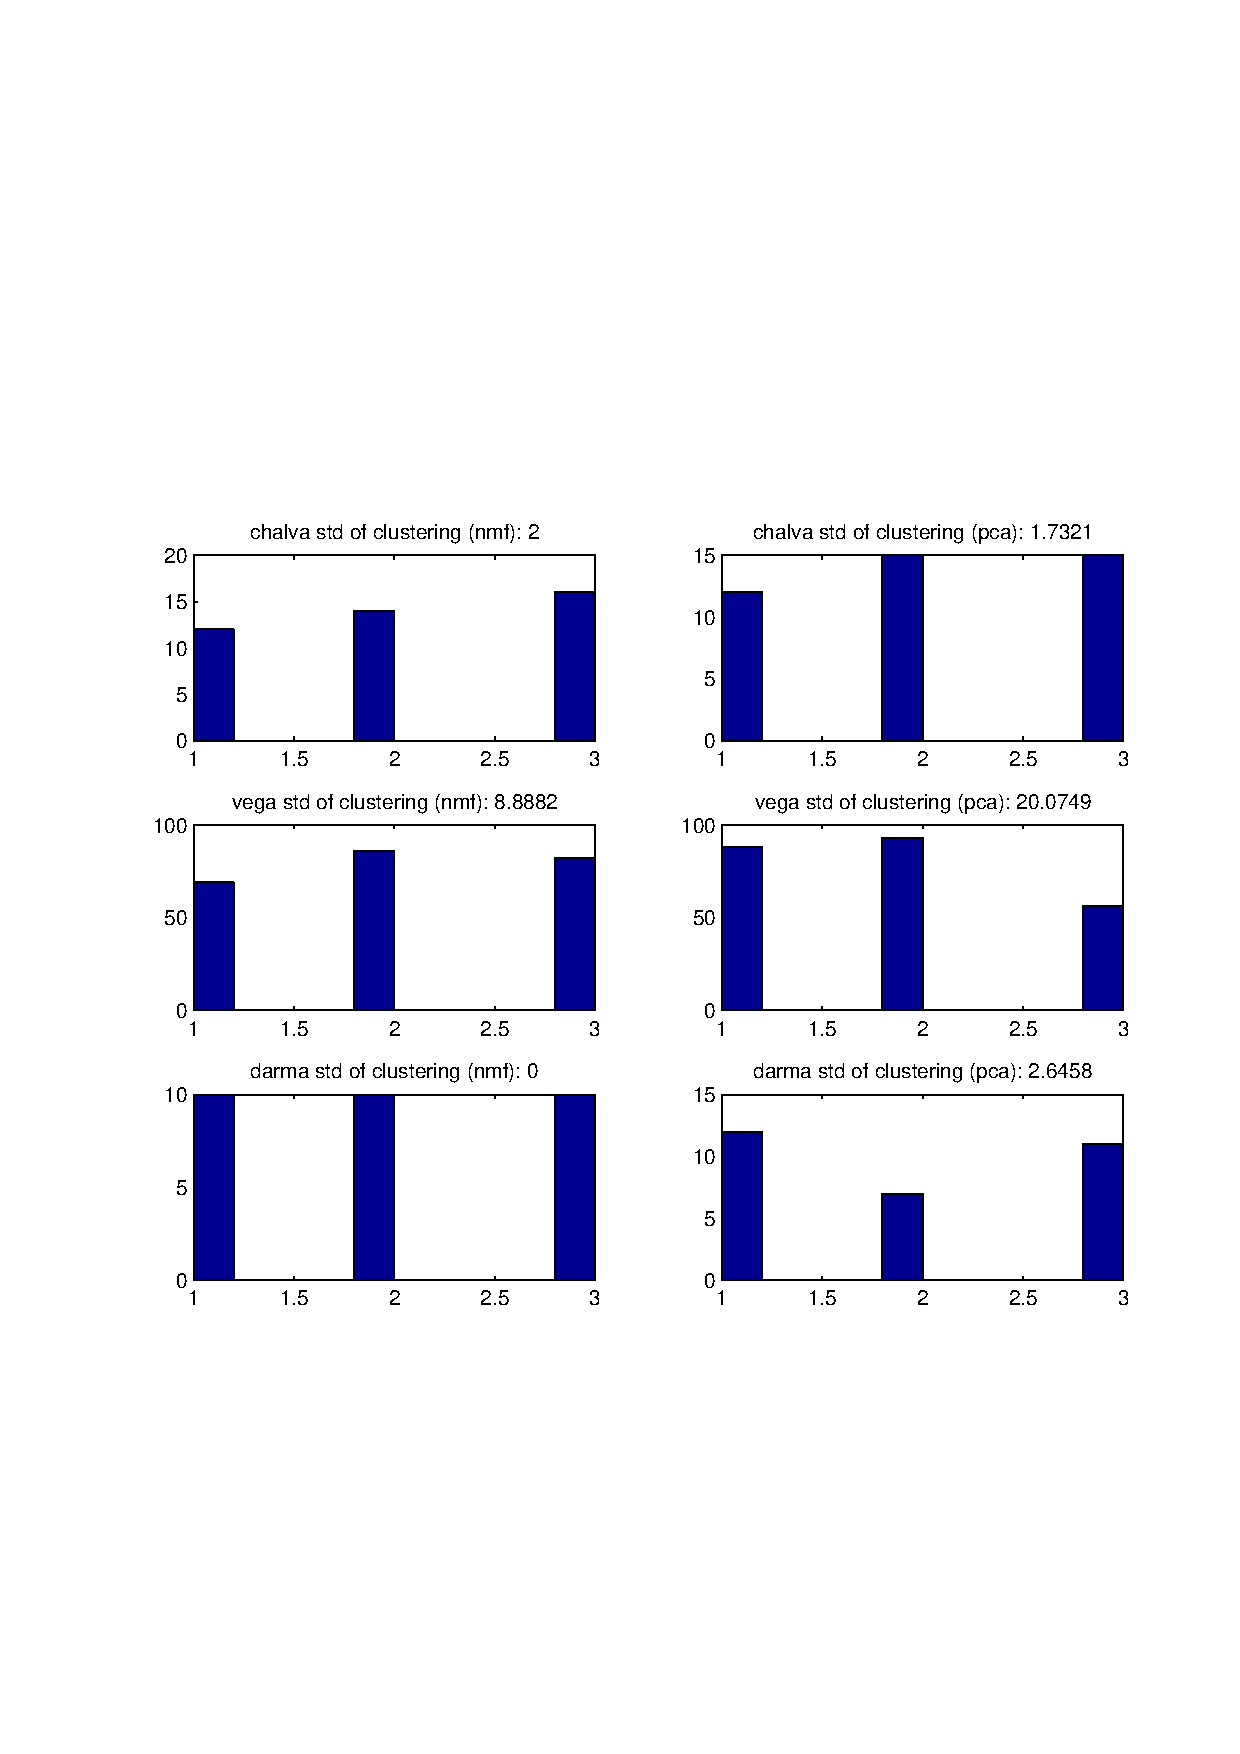
\includegraphics[width=0.8\textwidth]{images/syn_consist_sessions_std.pdf}
    \caption{Distribution and std of the group sizes when clustering the synergies obtained from different sessions}
    \label{sg:fig:images_syn_consist_sessions_std}
\end{figure}


% consist over sessions and method explanation plot (chalva)
\begin{figure}[ht]
    \centering
    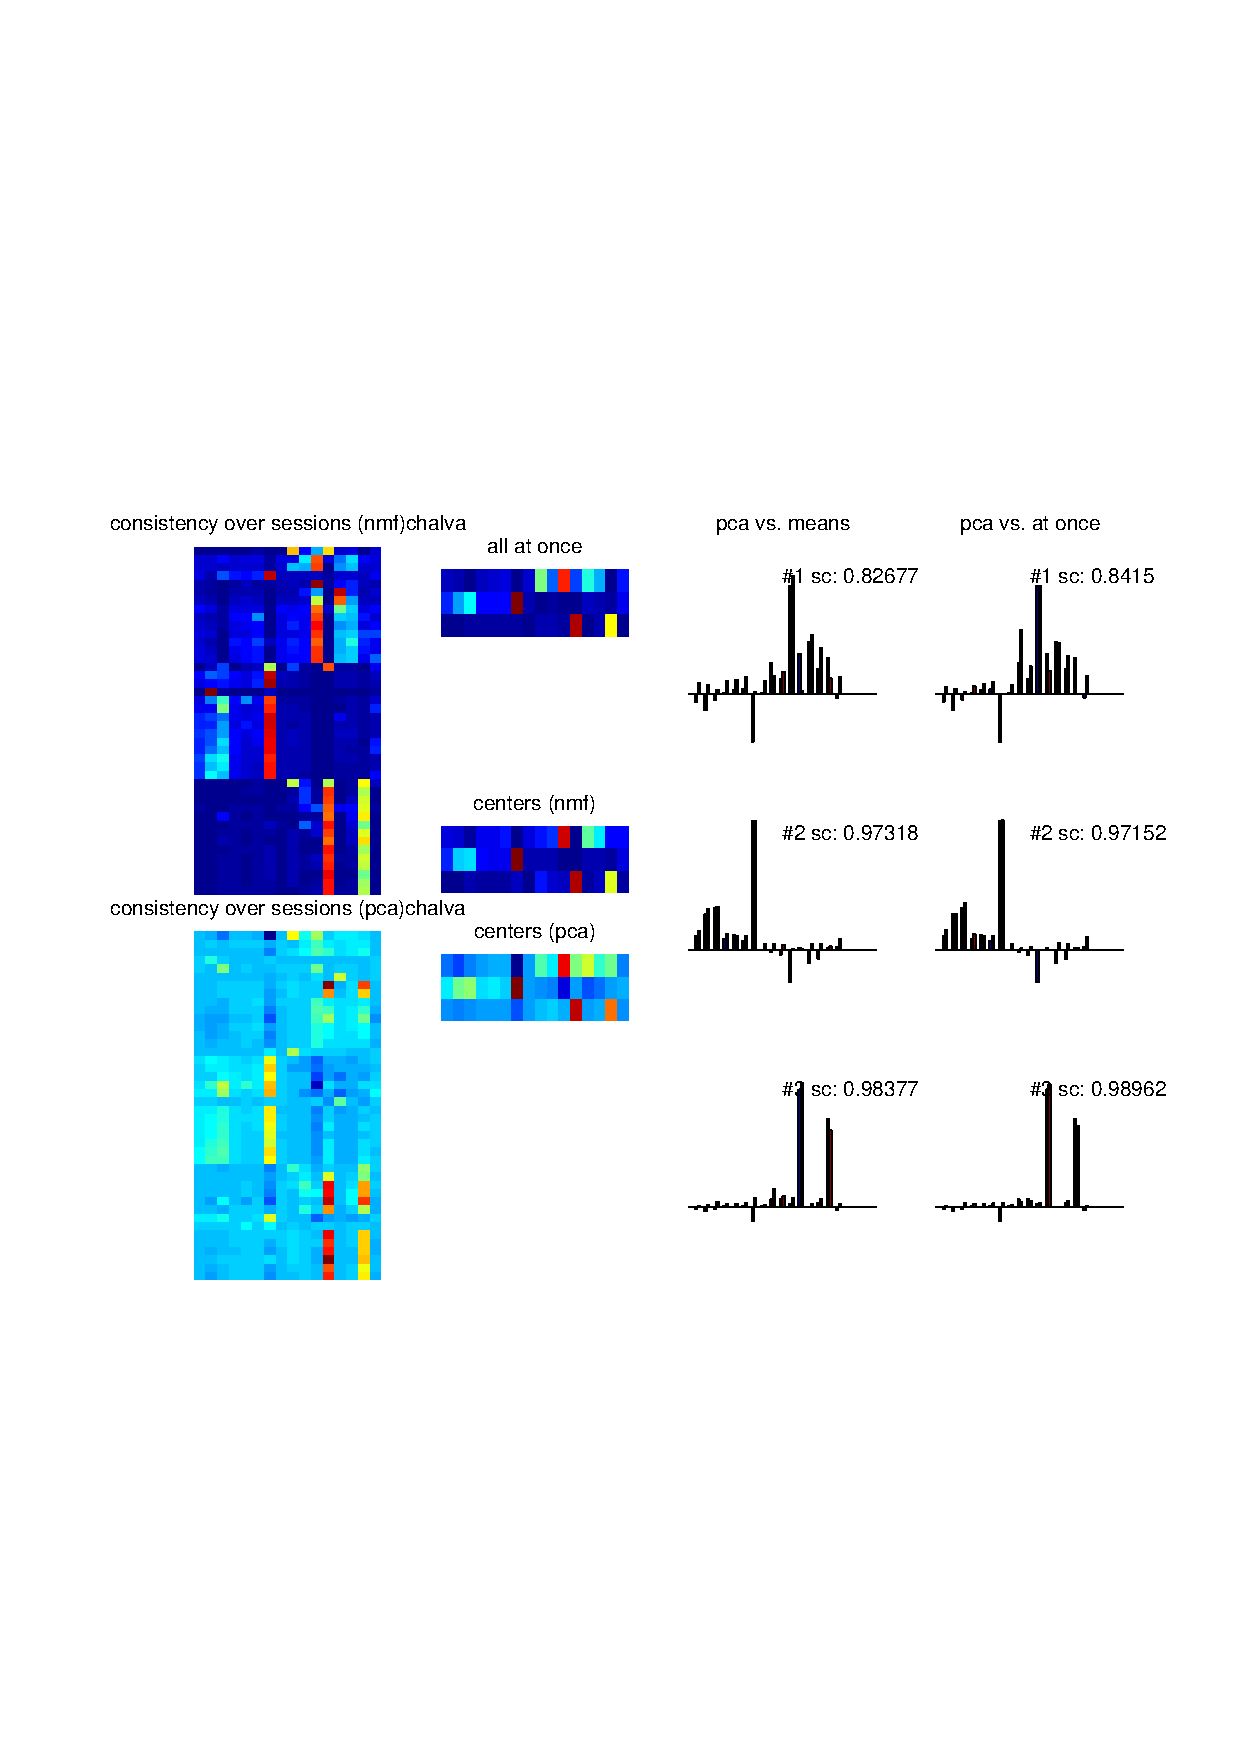
\includegraphics[width=0.8\textwidth]{images/syn_consist_sessions_chalva.pdf}
    \caption{
    all data in this plot is from pronation hand-position\\
    \textbf{a)} The stability of extracted synergies over sessions was assessed similar to the stability measure of the MF-algorithm~\rref{sg:fig:images_nmf_expl_stab3}. All results were pooled and clustered by a k-means algorithm with the number of prototypes corresponding to the number of synergies. Similarity within the three blocks demonstrates stability over sessions. The strength of activation is coded by color. Note that color-coding is distinct for NMF- and PCAICA extracted synergies as NMF gives only positive results.synergies sorted according to cluster membership for both methods\\
    \textbf{b)} comparison of cluster means and when computed the synergies on all data at once\\
    \textbf{c)} pca vs. nmf means\\
    \textbf{d)} pca vs. nmf all at once\\
    }
    \label{sg:fig:images_syn_consist_sessions_chalva}
\end{figure}

% summarizing table of nmf-pca and center-all similarities
\begin{table}[ht]
	\centering
	\begin{tabular}{r|c|c|c}
		\toprule
		                    & vega  & darma & chalva \\
		pca vs. nmf         &       &       & \\
		syn \#1              & 0.99  & 0.97  & 0.98\\
		syn \#2              & 0.98  & 0.98  & 0.97\\
		syn \#3              & 0.98  & 0.96  & 0.82\\
		\midrule
		mean vs. all        &       &       & \\
		syn \#1              & 0.98  & 0.91  & 0.99\\
		syn \#2              & -0.04 & 0.92  & 0.97\\
		syn \#3              & 0.88  & 0.95  & 0.84\\
		\bottomrule
	\end{tabular}
	\caption{}
	\label{sg:tab:syn_consist}
\end{table}


For subjects D and V data from 2 hand-positions was available. However, the synergies computed in separate conditions showed very strong similarity. 
\begin{figure}[ht]
    \centering
        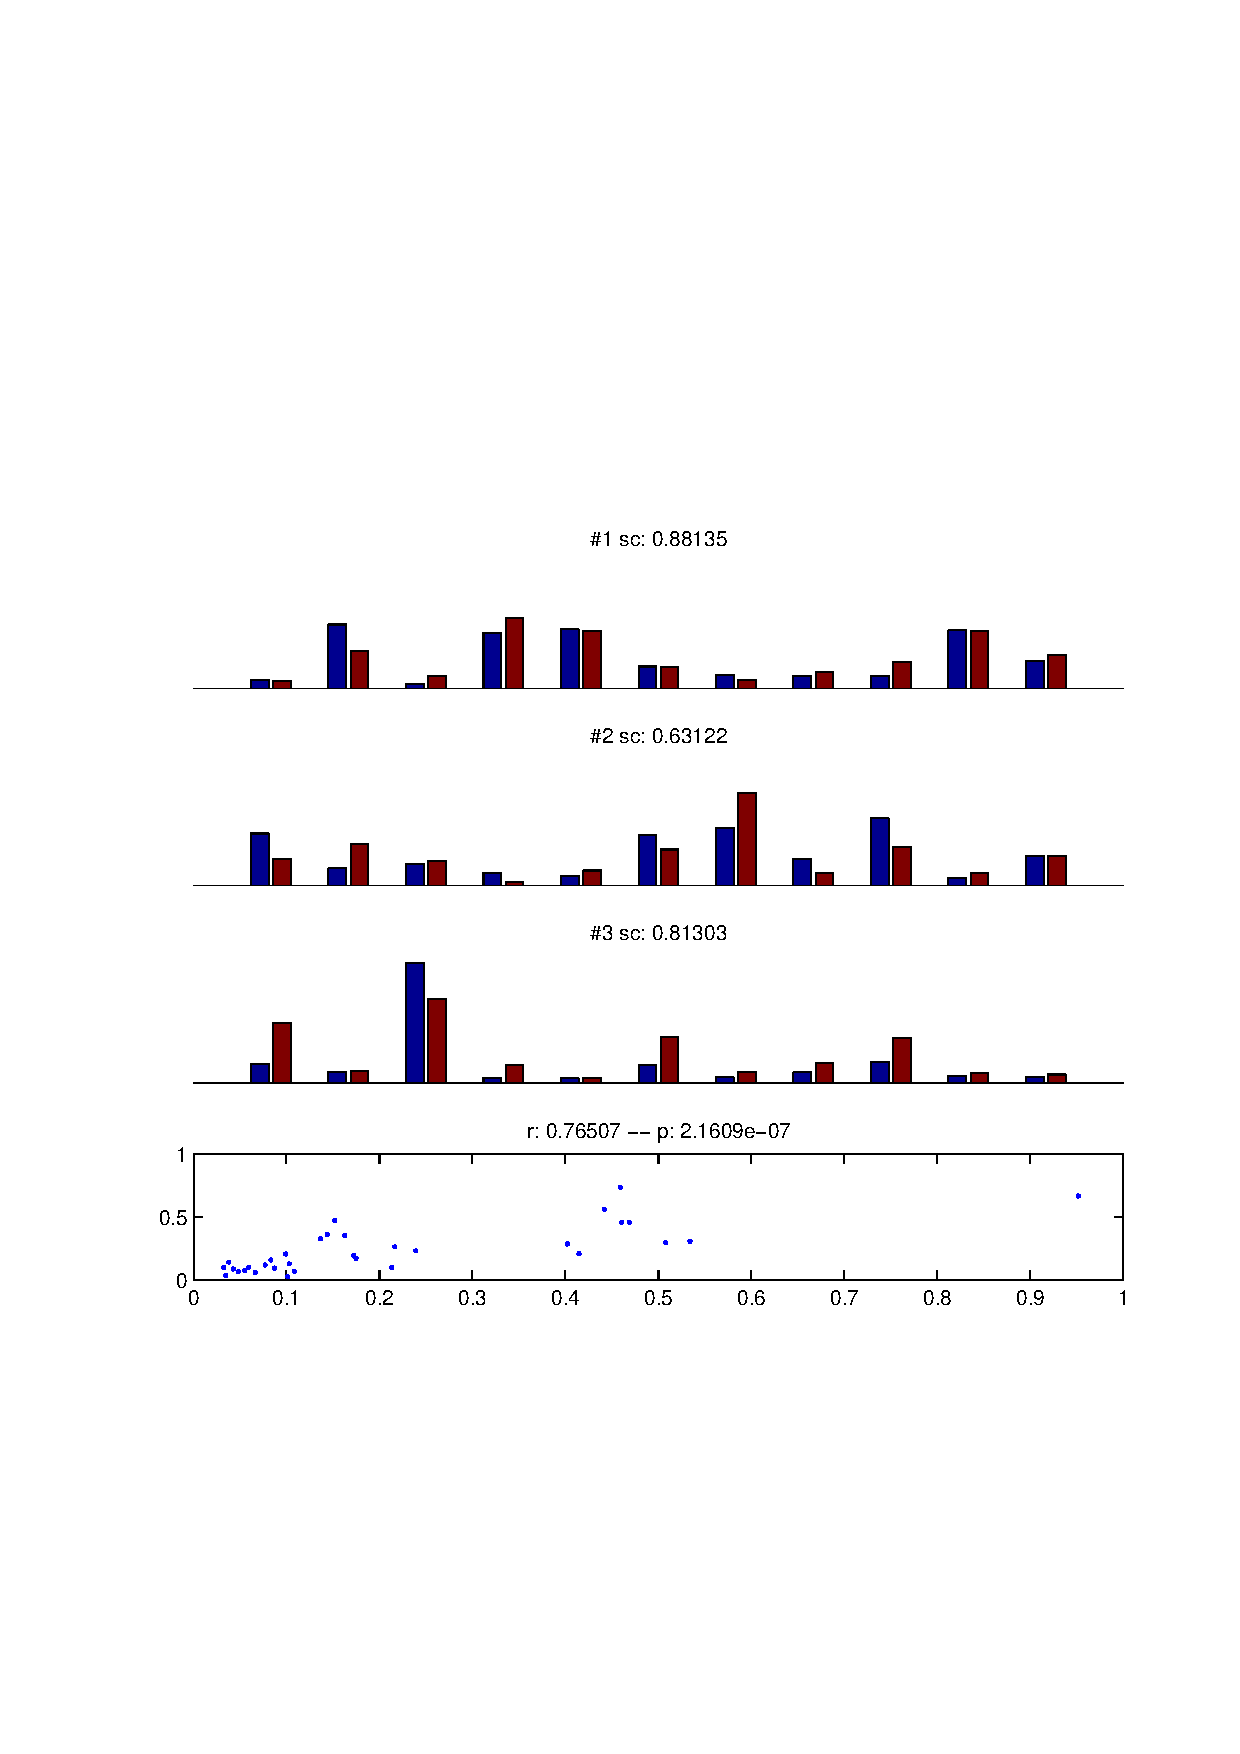
\includegraphics[width=0.8\textwidth]{images/post_consist_vega.pdf}
    \caption{Example of a posture similarity plot (subject V)}
    \label{sg:fig:images_post_consist_vega}
\end{figure}

\begin{figure}[ht]
    \centering
        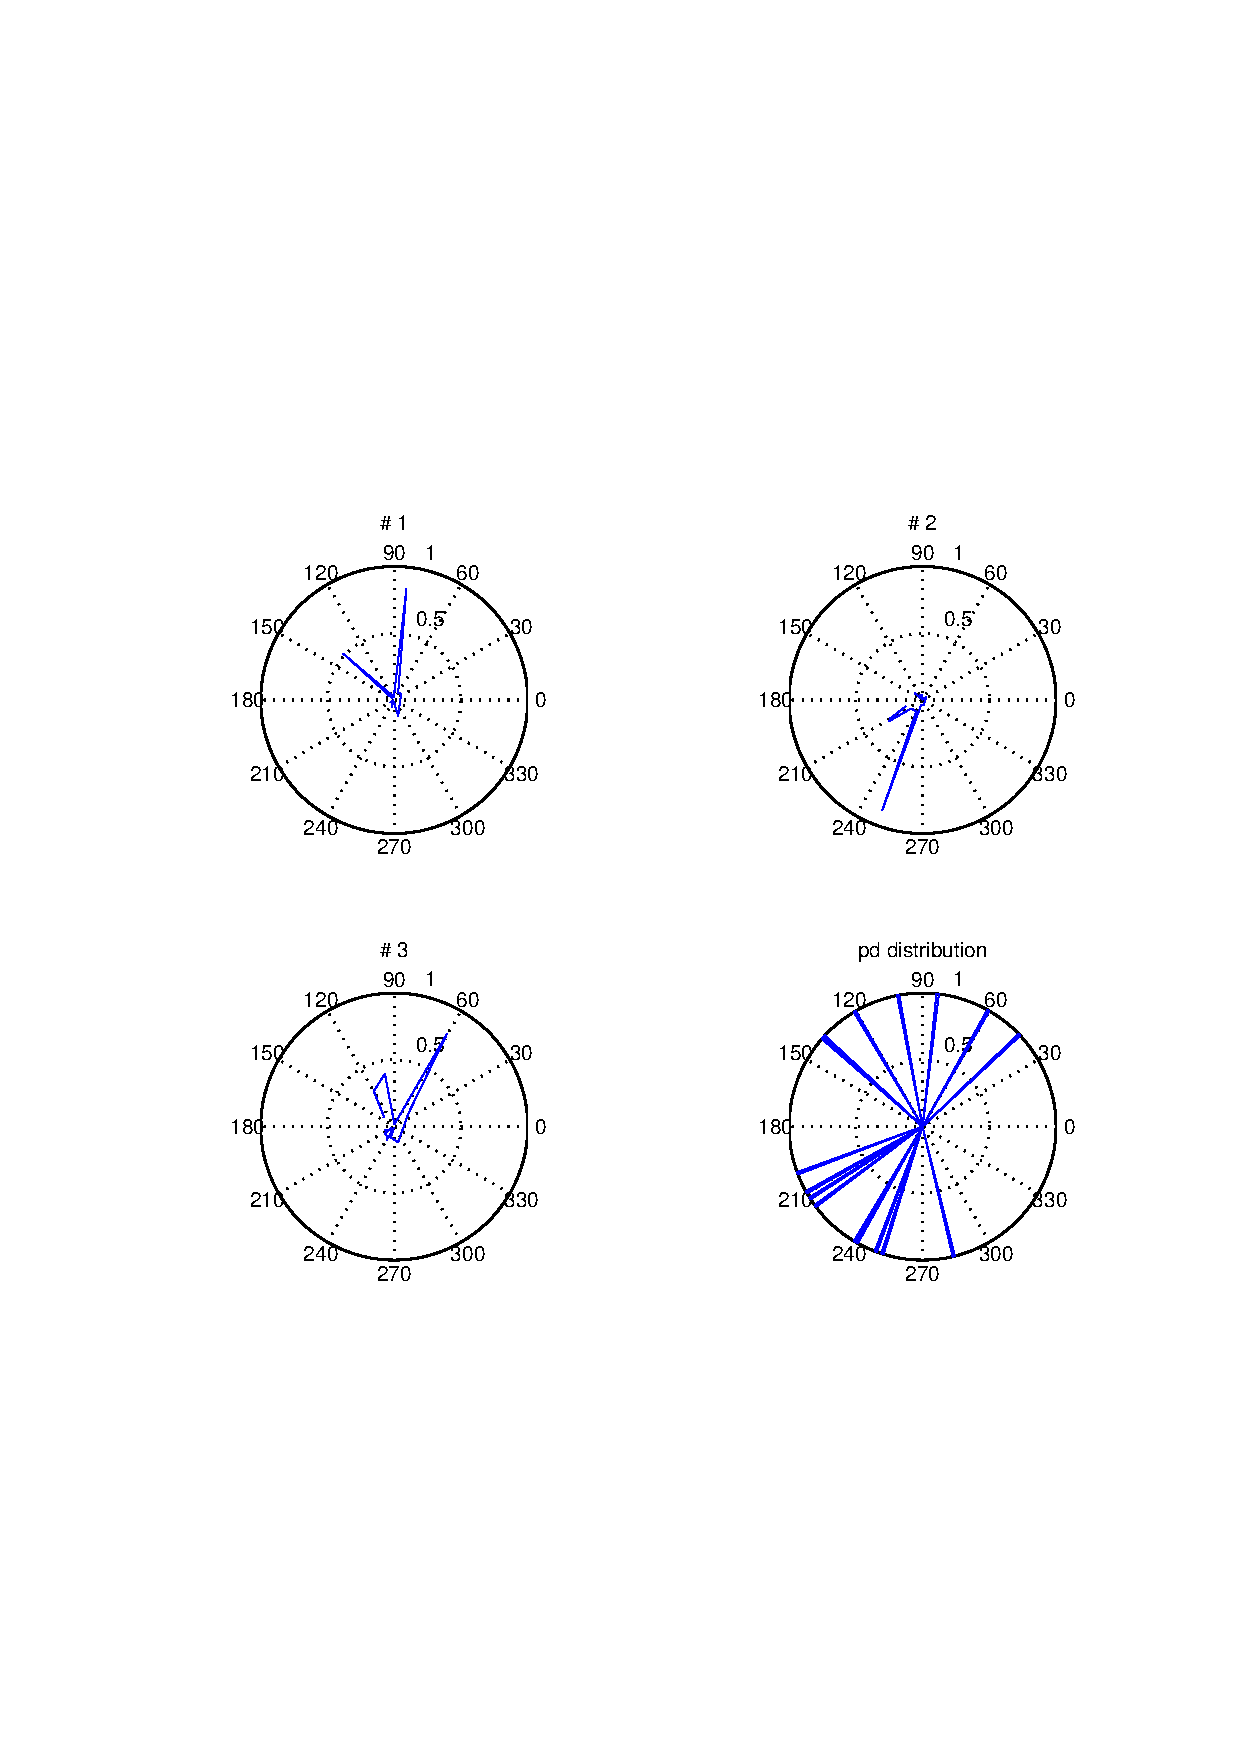
\includegraphics[width=0.8\textwidth]{images/syn_rose_pro_chalva.pdf}
    \caption{synergies in preferred directions (subject C)}
    \label{sg:fig:images_syn_rose_pro_chalva}
\end{figure}
\begin{figure}[ht]
    \centering
        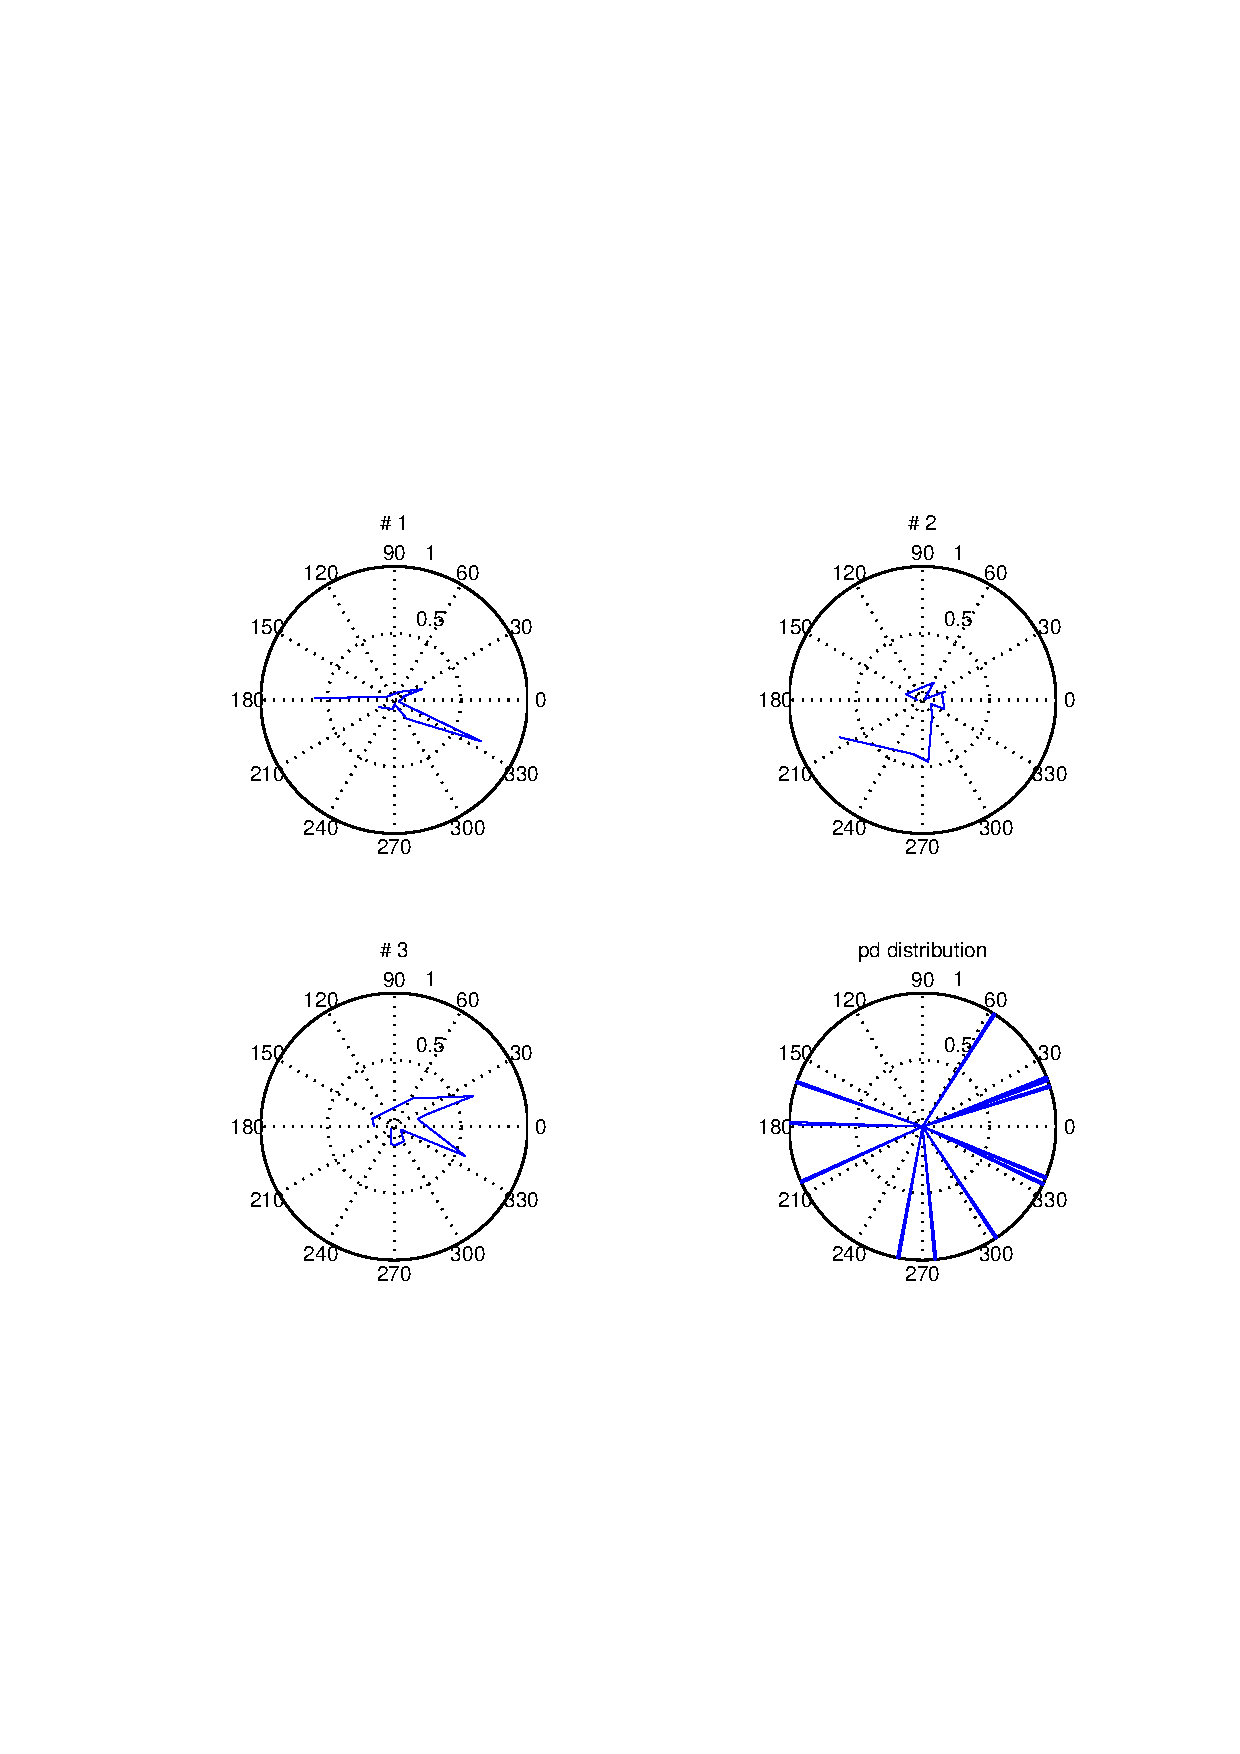
\includegraphics[width=0.8\textwidth]{images/syn_rose_pro_darma.pdf}
    \caption{synergies in preferred directions (subject D)}
    \label{sg:fig:images_syn_rose_pro_darma}
\end{figure}
\begin{figure}[ht]
    \centering
        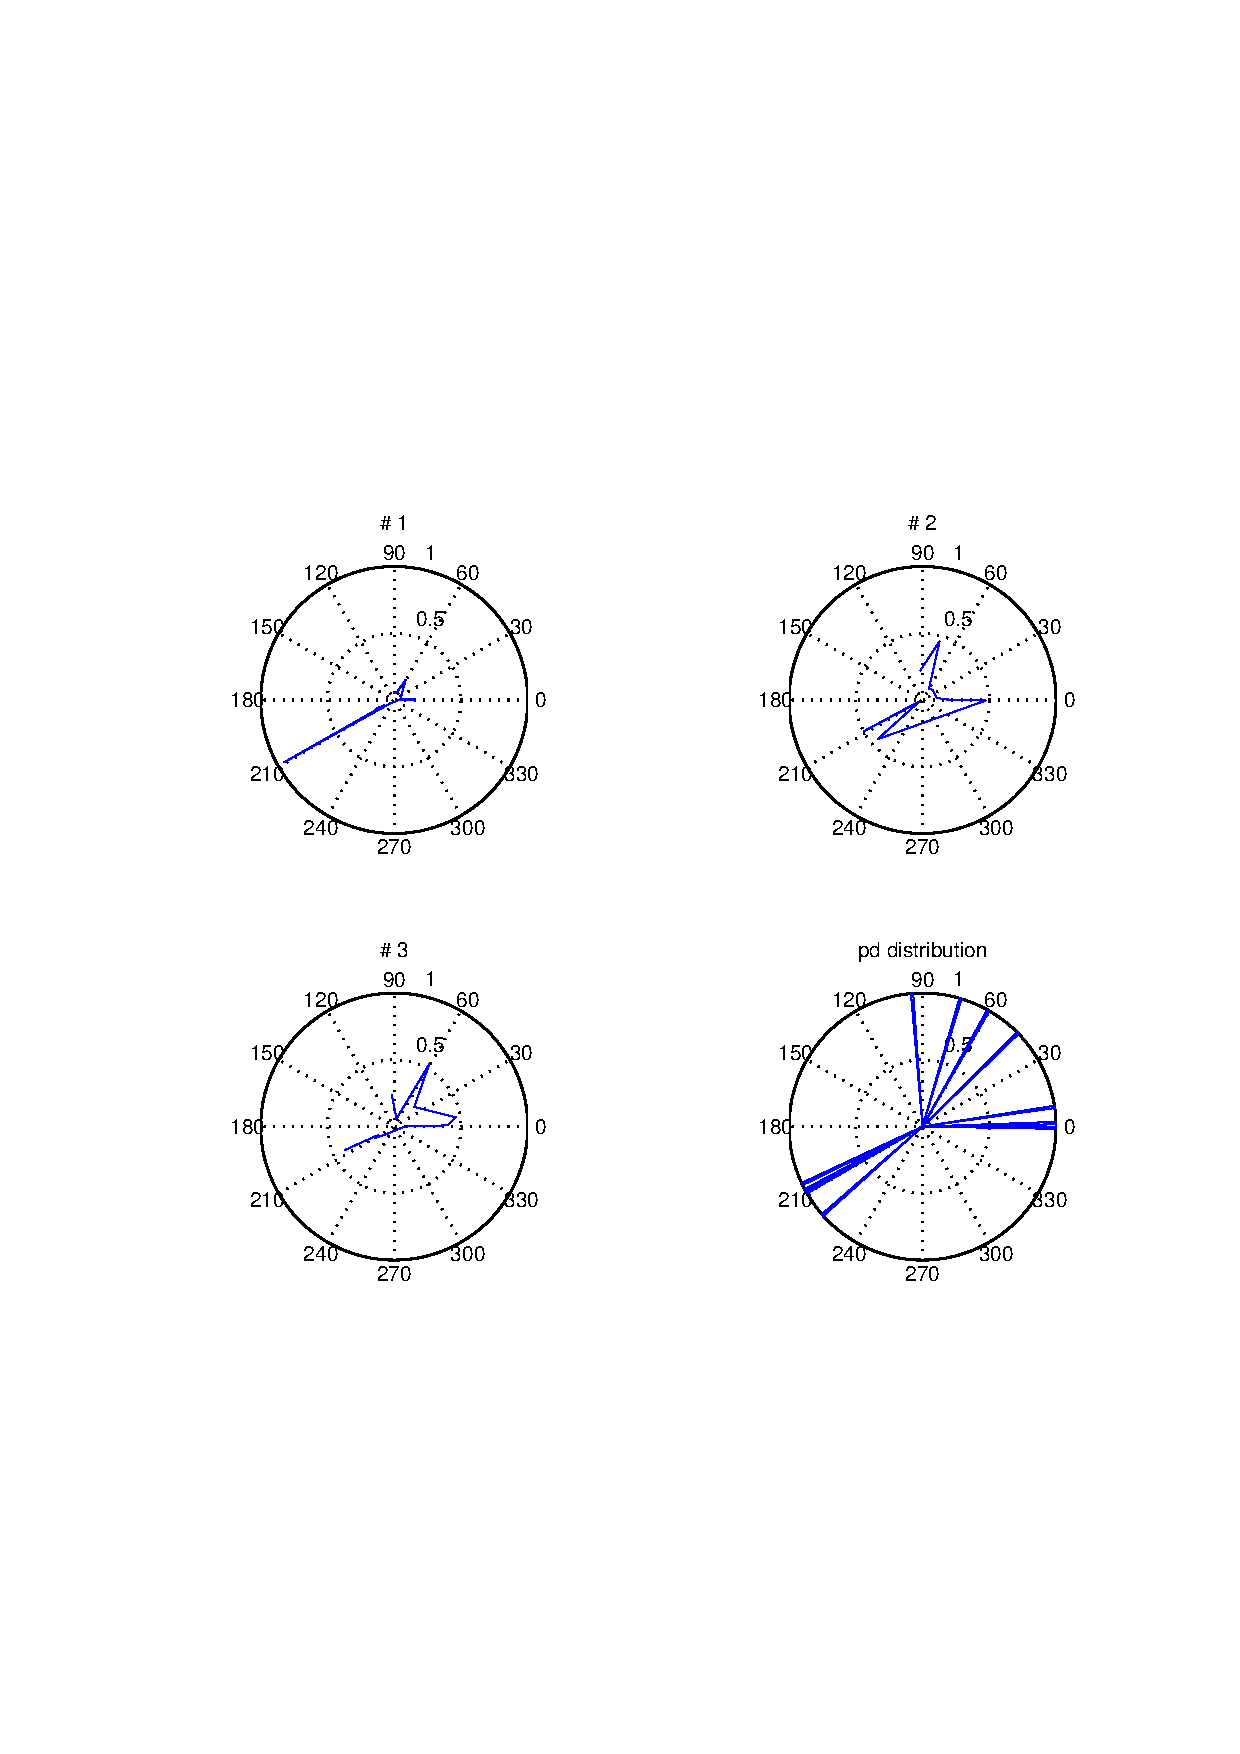
\includegraphics[width=0.8\textwidth]{images/syn_rose_pro_vega.pdf}
    \caption{synergies in preferred directions (subject V)}
    \label{sg:fig:images_syn_rose_pro_vega}
\end{figure}




It was thought that the circular standard deviation of muscle synergies in the space of preferred directions can be used to assess whether the result of matrix-factorization algorithms is realistic with respect to natural movement. The idea was that meaningful muscle activation patterns should have a lower \emph{cstd} than random activation patters in order to initiate movement in certain directions. The \emph{cstd} was computed on the average synergies of all single sessions by the method explained in Section~\ref{sg:sub:pd}. For none of these synergies a significantly smaller circular standard deviation than for random data was found \rref{sg:fig:images_circ_std_syns}.
As the PDs proved to be significant and the synergies were stably extracted by different algorithms, the reason for this result has to be found within the directedness measurement or in the this measurement underlying assumptions that muscle activation patterns correspond to directed movement. Within the current approach, a lot of averaging takes place during computation. First the PD for a muscle is computed by a vector summation, then this PD is averaged over all significant session
and finally this computed PD is assigned to a muscle in an activation pattern,
only scaled in length by the value of the activation. As a lot of information is lost within this process,
direct basis approaches or probabilistic methods might be more promising.
However, it could also be that the assumption that meaningful muscle activation patterns should correspond to
directed movement is completely wrong. There could be a meaningful muscle activation pattern
which has two modes of activation each pointing to a different point in space.
The purpose of this muscle co-activation into opposing directions could be to increase
joint stiffness. In this case the circular variance will be very high, but the synergy would be still meaningful. 
More promising measures for the meaningfulness of muscle activation patterns will be proposed in the outlook part
of this thesis.
\begin{figure}[ht]
    \centering
        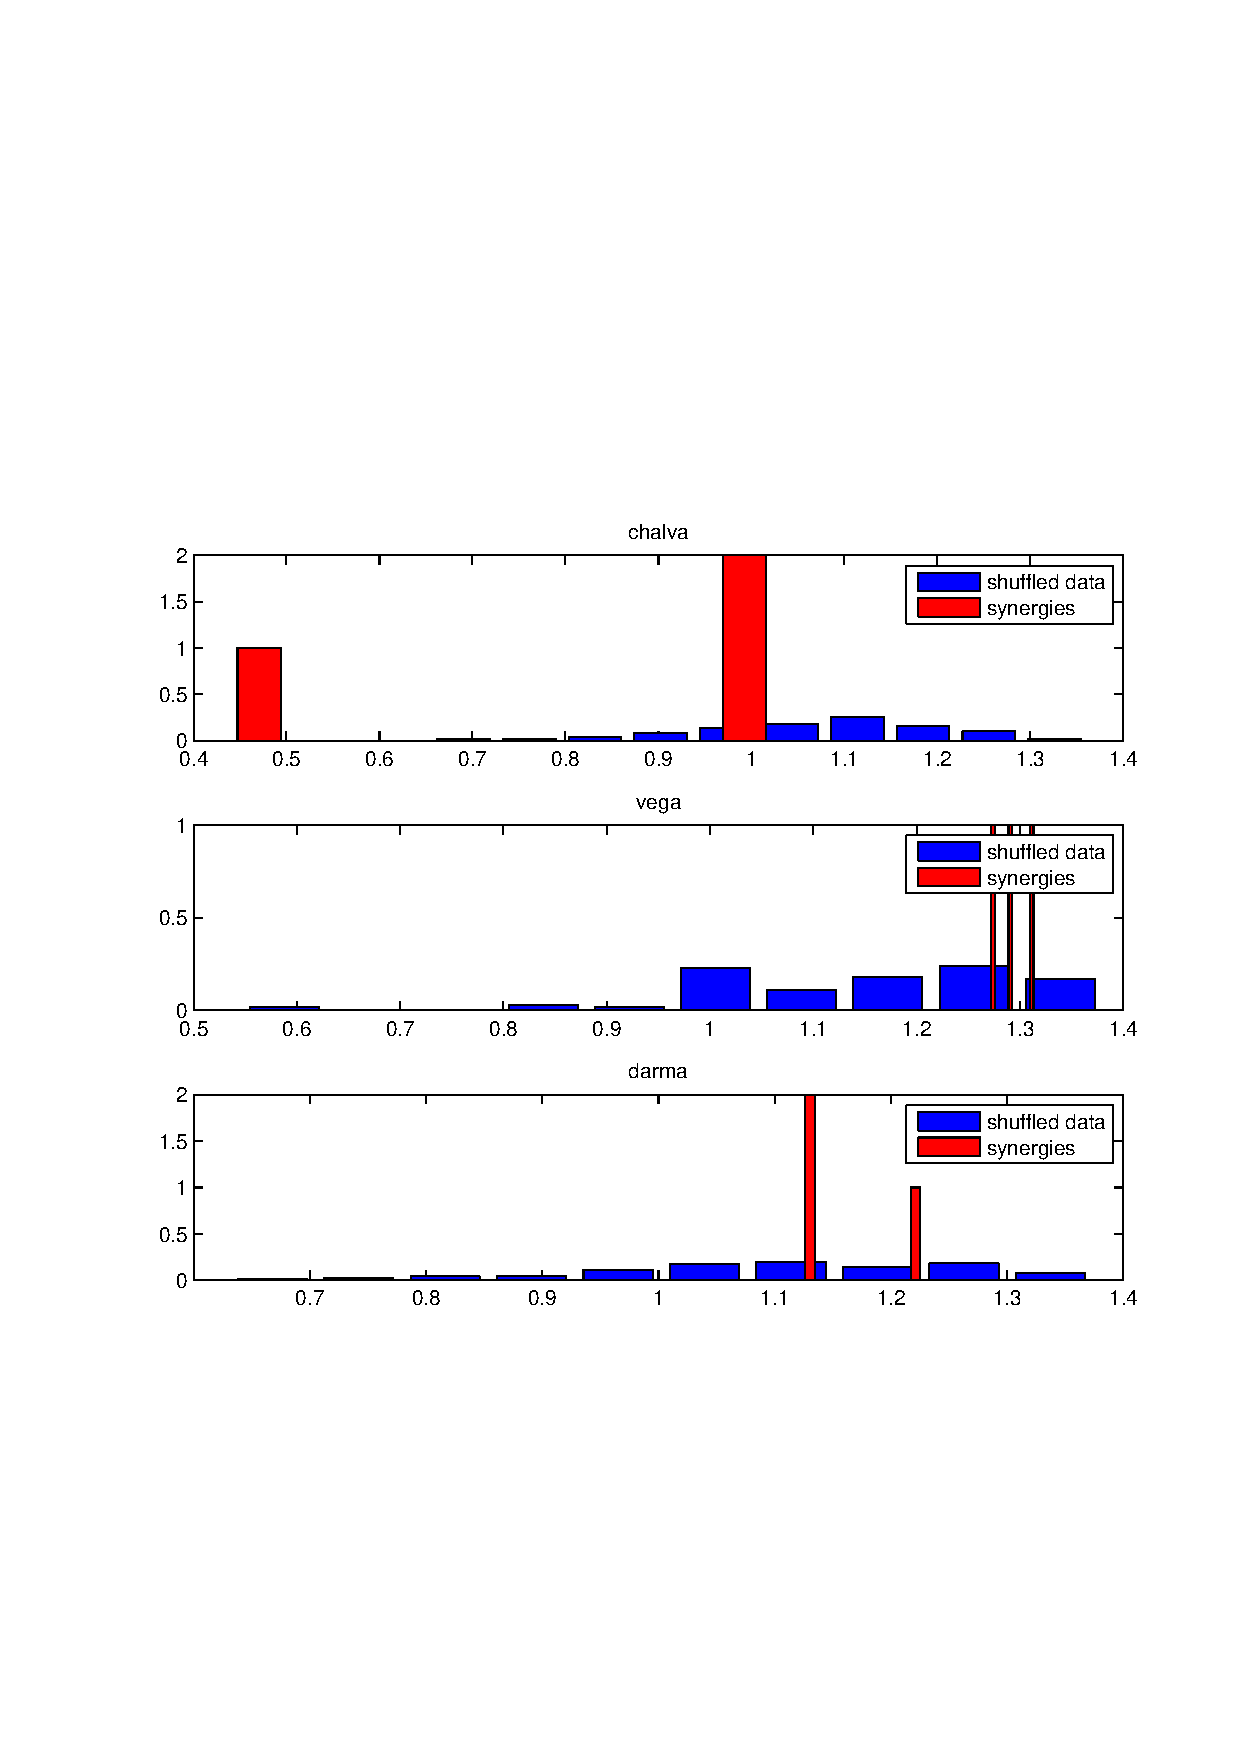
\includegraphics[width=0.8\textwidth]{images/circ_std_syns.pdf}
    \caption{This plot investigates whether the found synergies are more \emph{directed} than random data with the same statistical properties. Random activation patterns drawn from the values of single session synergies are compared with the average synergies over all sessions. For all three monkeys it does not seam as the synergies are more directed than by chance.}
    \label{sg:fig:images_circ_std_syns}
\end{figure}

To sum up, it was possible to extract 3 muscle synergies from data, which was collected from many sessions of natural movement. The extracted synergies proved to be similar over different hand postures and were reliably found from different algorithms of matrix factorization. This is consistent with the findings of other publications that were mentioned in the introduction.



%output off all remaining pictures of this section
\afterpage{\clearpage}

% section nat_mov_syns (end)


% 1
% ===============================================================
% = analysis if synergies from respones to cortical stimulation =
% ===============================================================
\section{Patterns in the evoked responses} % (fold)
\label{sg:sec:evoked_syns}

Within the recording-sessions for which EMG data was available (C: 15, V: 91), in some sub-sessions (C: 64, V: 157) cortical microstimulation in different sites took place for two of the subjects. For each sub-session average response windows around stimulation time were computed and after visual inspection the sub-sessions containing artifacts in the window were sorted out as well as sub-sessions with a muscle field size of 0 (no significant response). 
% table of all available data 
\begin{table}[ht]
	\centering
	\begin{tabular}{r|cc|cc}
		\toprule
		                    & \multicolumn{2}{c}{vega}  & \multicolumn{2}{c}{chalva}  \\
	    \midrule
		total sub-sessions  & \multicolumn{2}{c}{157}   & \multicolumn{2}{c}{64}    \\
		artifact            & \multicolumn{2}{c}{24}    & \multicolumn{2}{c}{0}        \\
		zero response field & \multicolumn{2}{c}{19}    & \multicolumn{2}{c}{20}       \\
		\bottomrule
		remaining           & \multicolumn{2}{c}{114}   & \multicolumn{2}{c}{44}       \\
		                    & pronation & supination    & pronation & supination \\
		separate            & 62        & 50            & 44        & 0         \\
		\bottomrule
	\end{tabular}
	\caption{}
	\label{sg:tab:sorting_table_evoked}	
\end{table}

As described before, arm-related areas were mapped by trains of stimulating pulses and the observation of visible responses (jerking of muscles) to this stimulation. This method could serve only for very coarse mapping as muscle activation is not necessarily visible. Therefore muscle field sizes of responses were calculated which give a more objective method for detection of arm-related locations in the cortex. For subject V data was recorded in pronation and supination hand-position.
A distribution of muscle field size can be seen in figure~\rref{sg:fig:images_responses} together with a plot of the muscle field size in relation to stimulation site. In this plot it becomes visible that the preliminary coarse mapping is not perfectly reliable as even sites that showed facial or no response can have significant and large muscle fields. However muscle fields are generally larger in stimulation sites mapped to finger or wrist movements. 
\begin{figure}[ht]
    \centering
        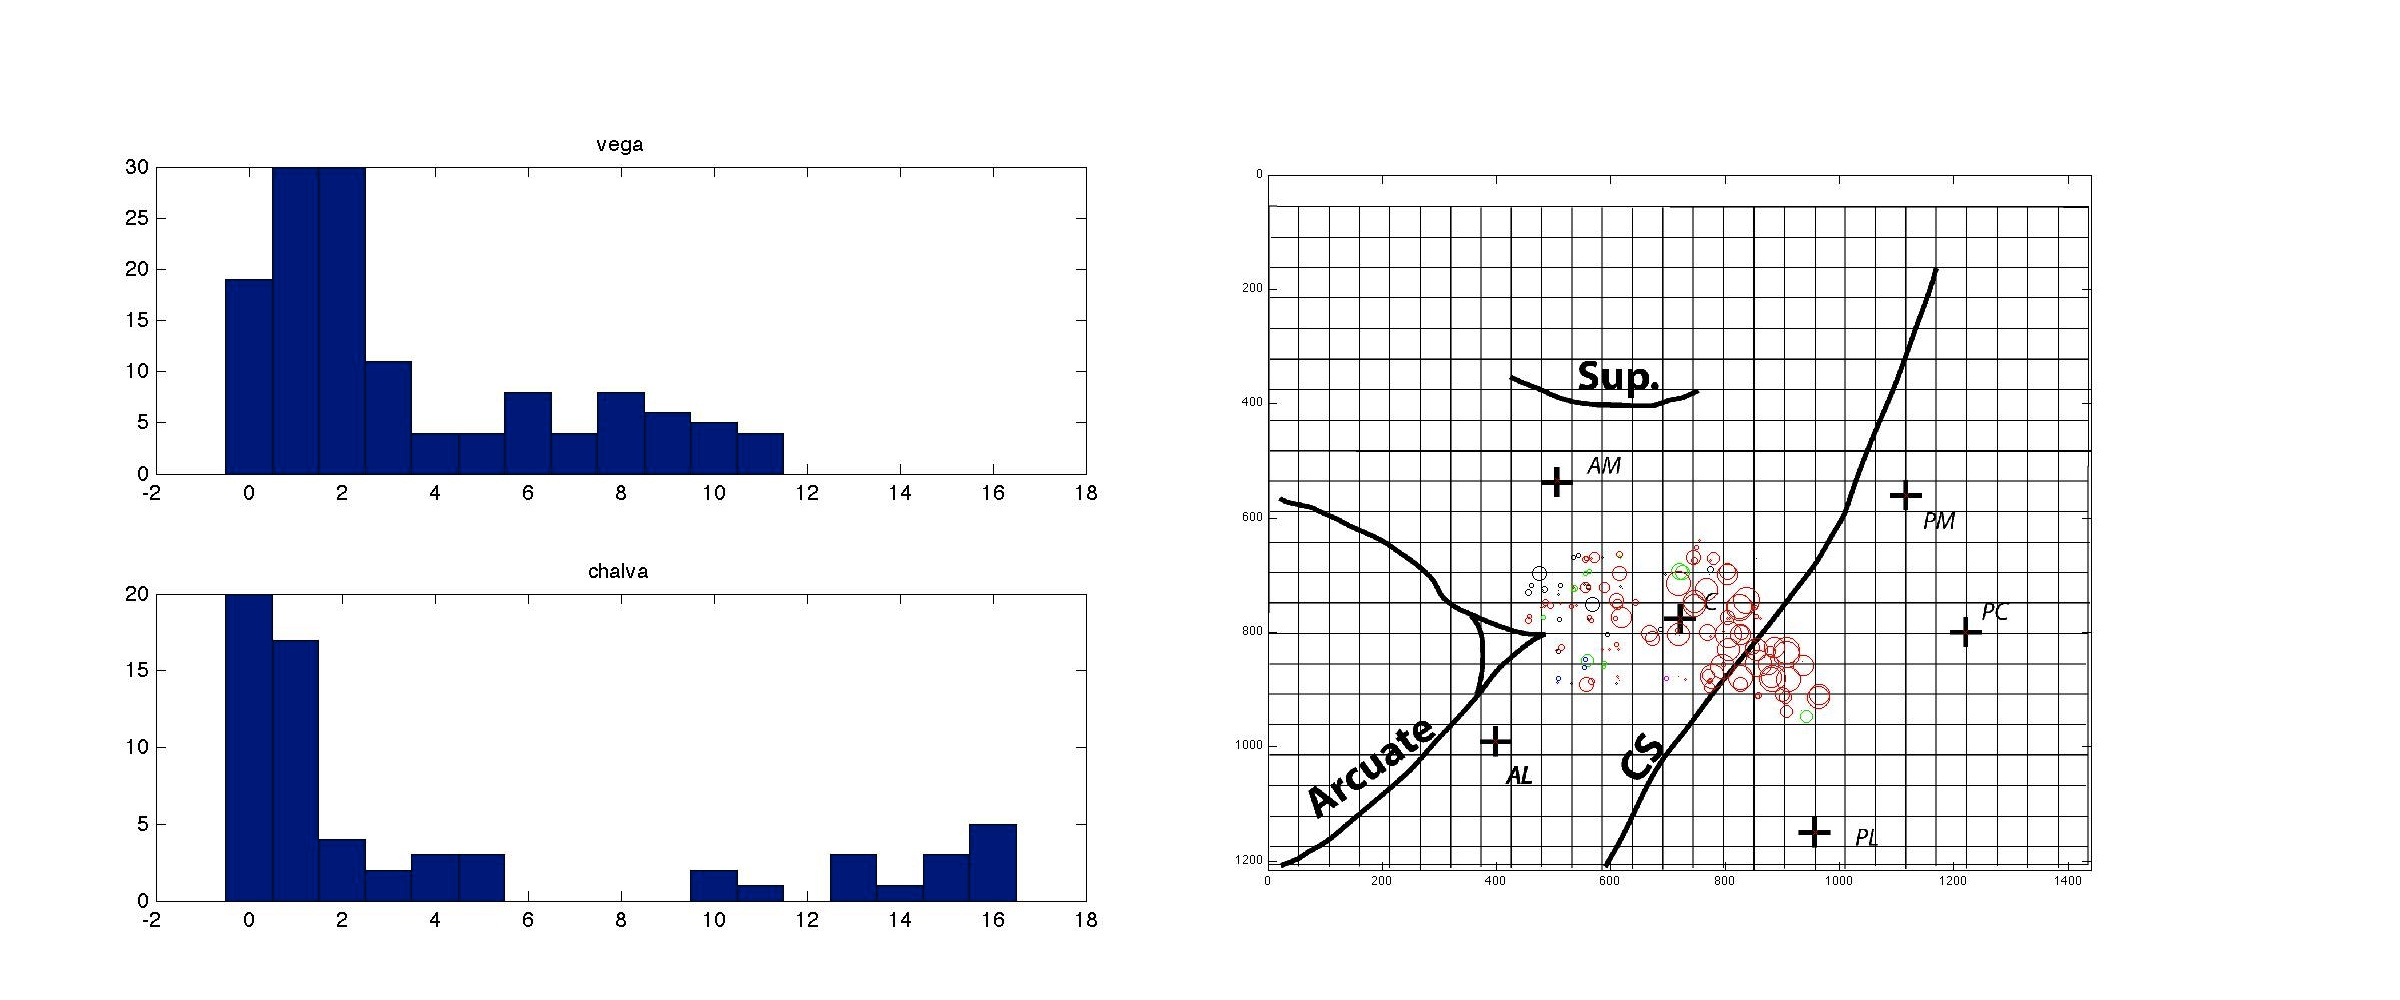
\includegraphics[width=\textwidth]{images/responses.jpg}
    \caption{The distribution of muscle field size and the relation between muscle field size and the site of stimulation. Note that even sites that showed observable responses in facial areas during the coarse mapping might exhibit significant muscle fields.}
    \label{sg:fig:images_responses}
\end{figure}

In each location, single pulse stimulation was applied with different stimulation amplitudes (from minimum 50 up to 250 $\mu A$) but not in all locations with all amplitudes. For each location the stimulation amplitude closest to $150 \mu A$ was chosen as most data was available around this strength~\rref{sg:fig:stimamp_dist} \emph{c}. Please notice that these are single pulse stimulations in contrast to the 50 ms \@ 300 Hz used for the mapping of the cortical surface.

% figure of stim amp distribution
\begin{figure}[ht]
	\centering
		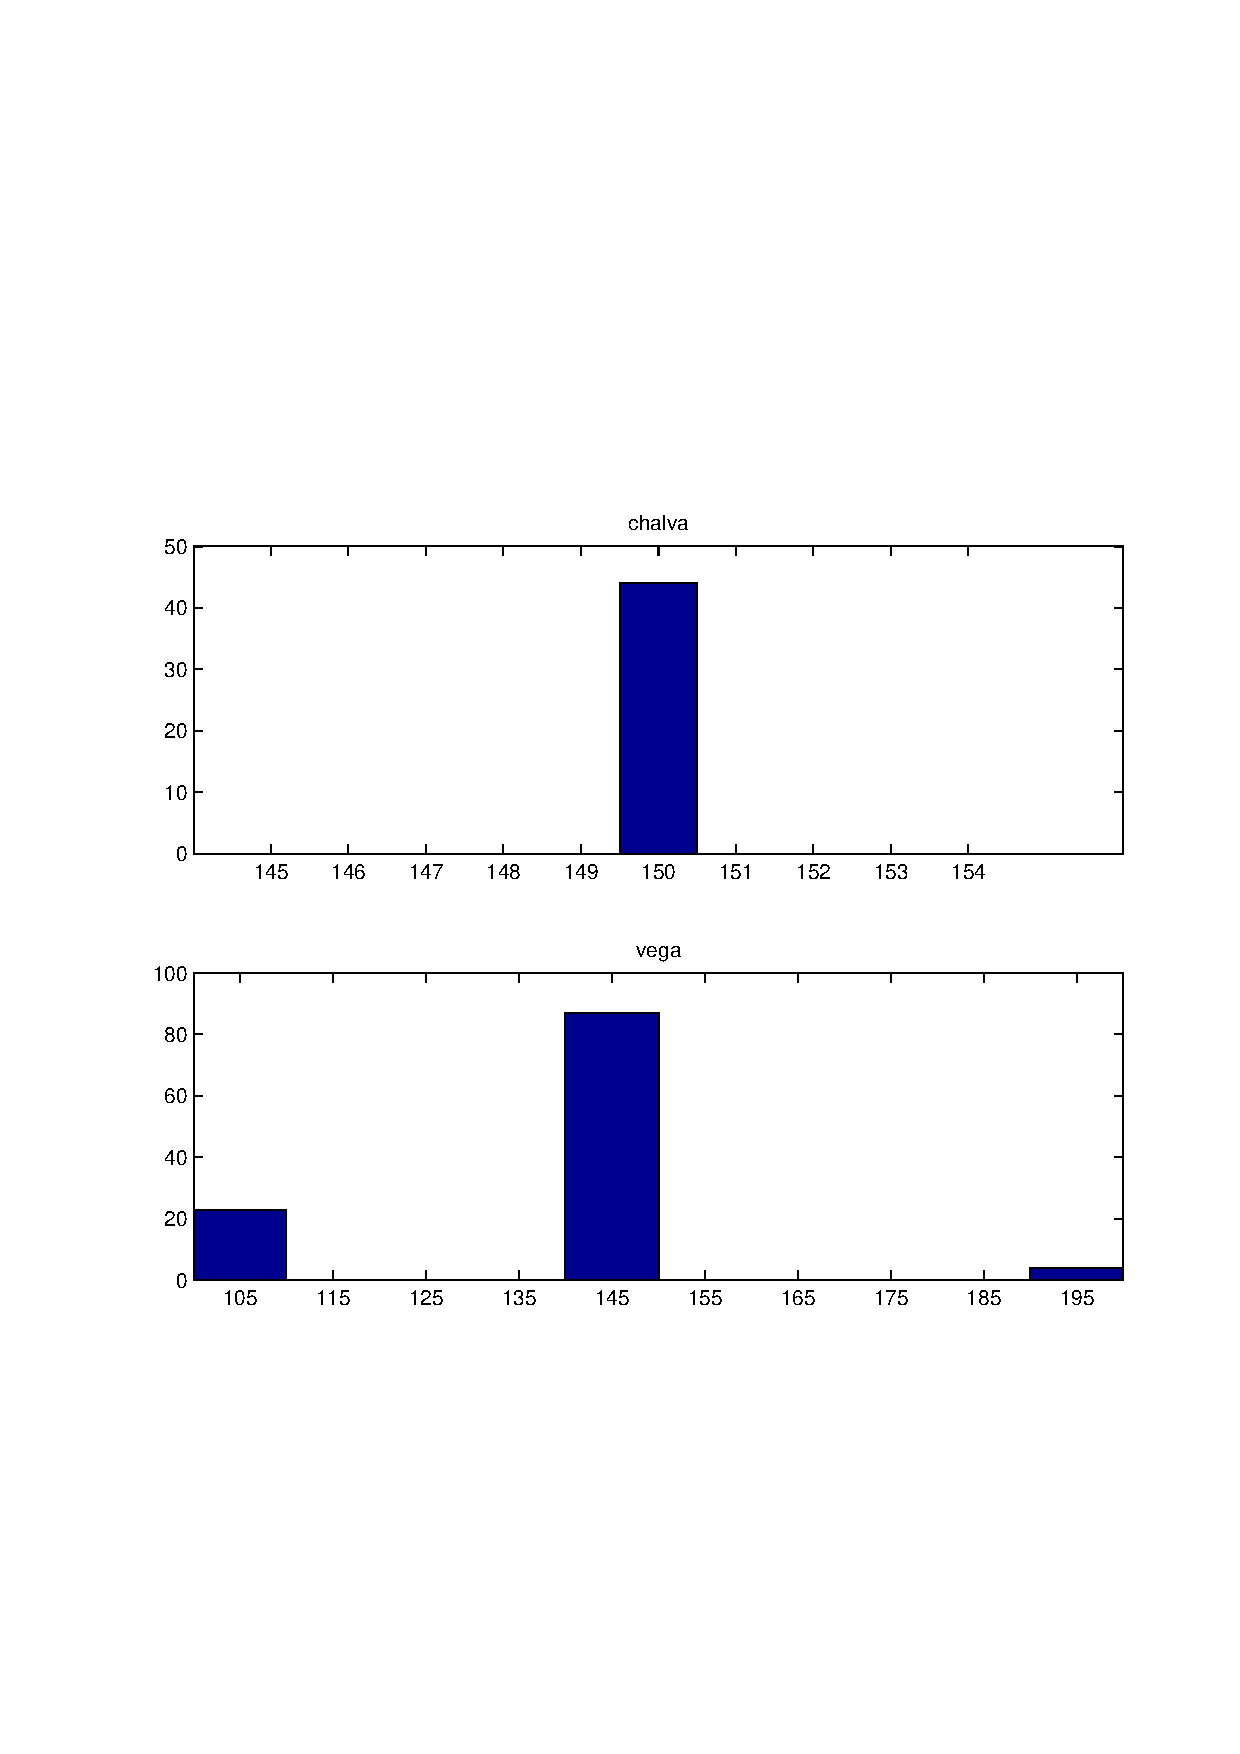
\includegraphics[width=0.5\textwidth]{images/stim_amp_dist.pdf}
	\caption{
		For each location the stimulation amplitude closest to $150 \mu A$ was chosen. The distribution shows the actually chosen stimulation amplitudes as $150 \mu A$ was not available for all locations.}
	\label{sg:fig:stimamp_dist}
\end{figure}
\begin{figure}[ht]
    \centering
        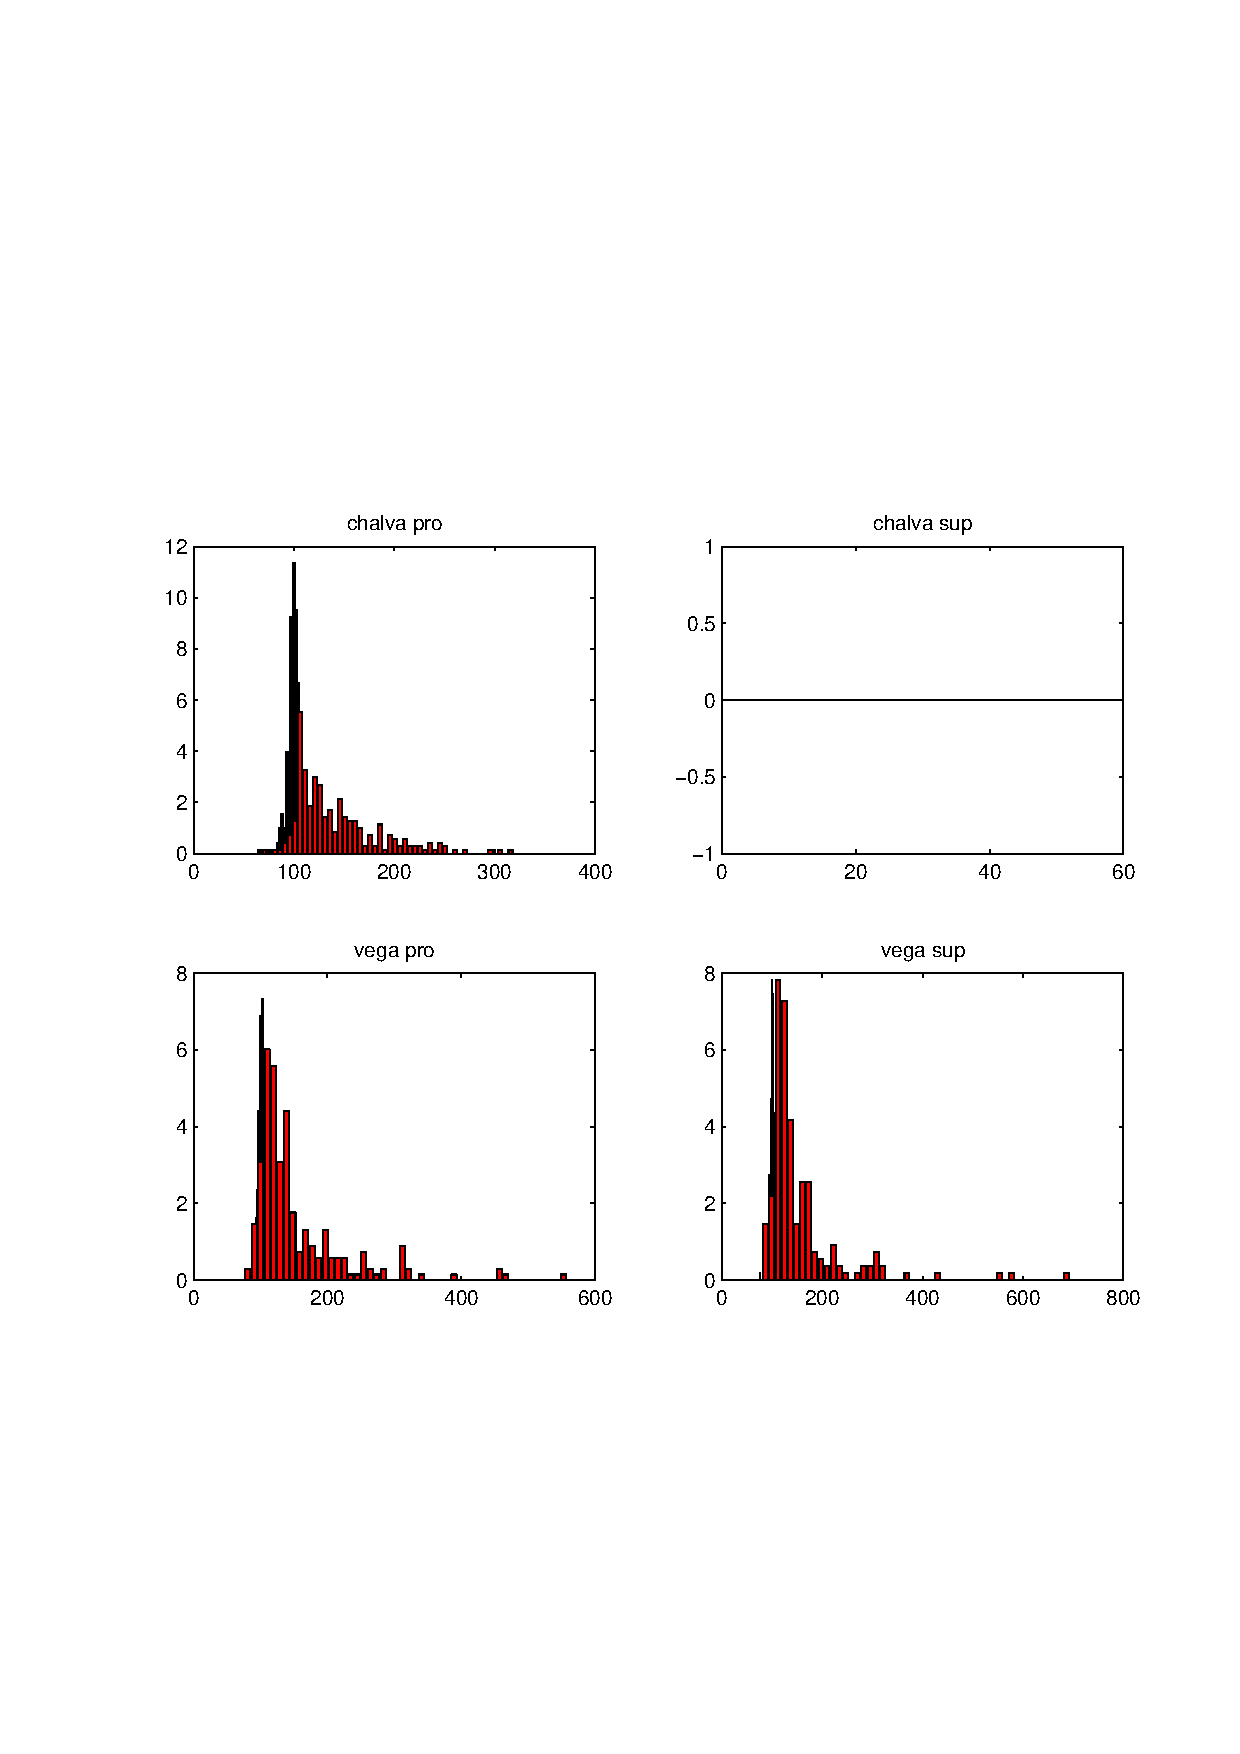
\includegraphics[width=0.8\textwidth]{images/response_dist.pdf}
    \caption{Distribution of response values. The part of the distribution which is colored red are the values from significant responses.}
    \label{sg:fig:images_response_dist}
\end{figure}


For each subject we calculated the fraction of stimulations for which the response field was 0 (C: 0.31 V: 0.14286). The plot of response fields and the distribution of actual responses shows that the stimulation induced responses result in a sparse matrix. Therefore we did not calculate synergies on this data by applying MF-algorithms. In contrast a simple kmeans clustering was used in order to look for structure in the data. A plot of mean distance of a cluster prototype to its assigned data-points suggest to look for three clusters. For subject V where both hand-positions were available no influence of the posture on the evoked responses can be found. Three clearly distinct clusters can be found for both subjects
\begin{figure}[ht]
    \centering
        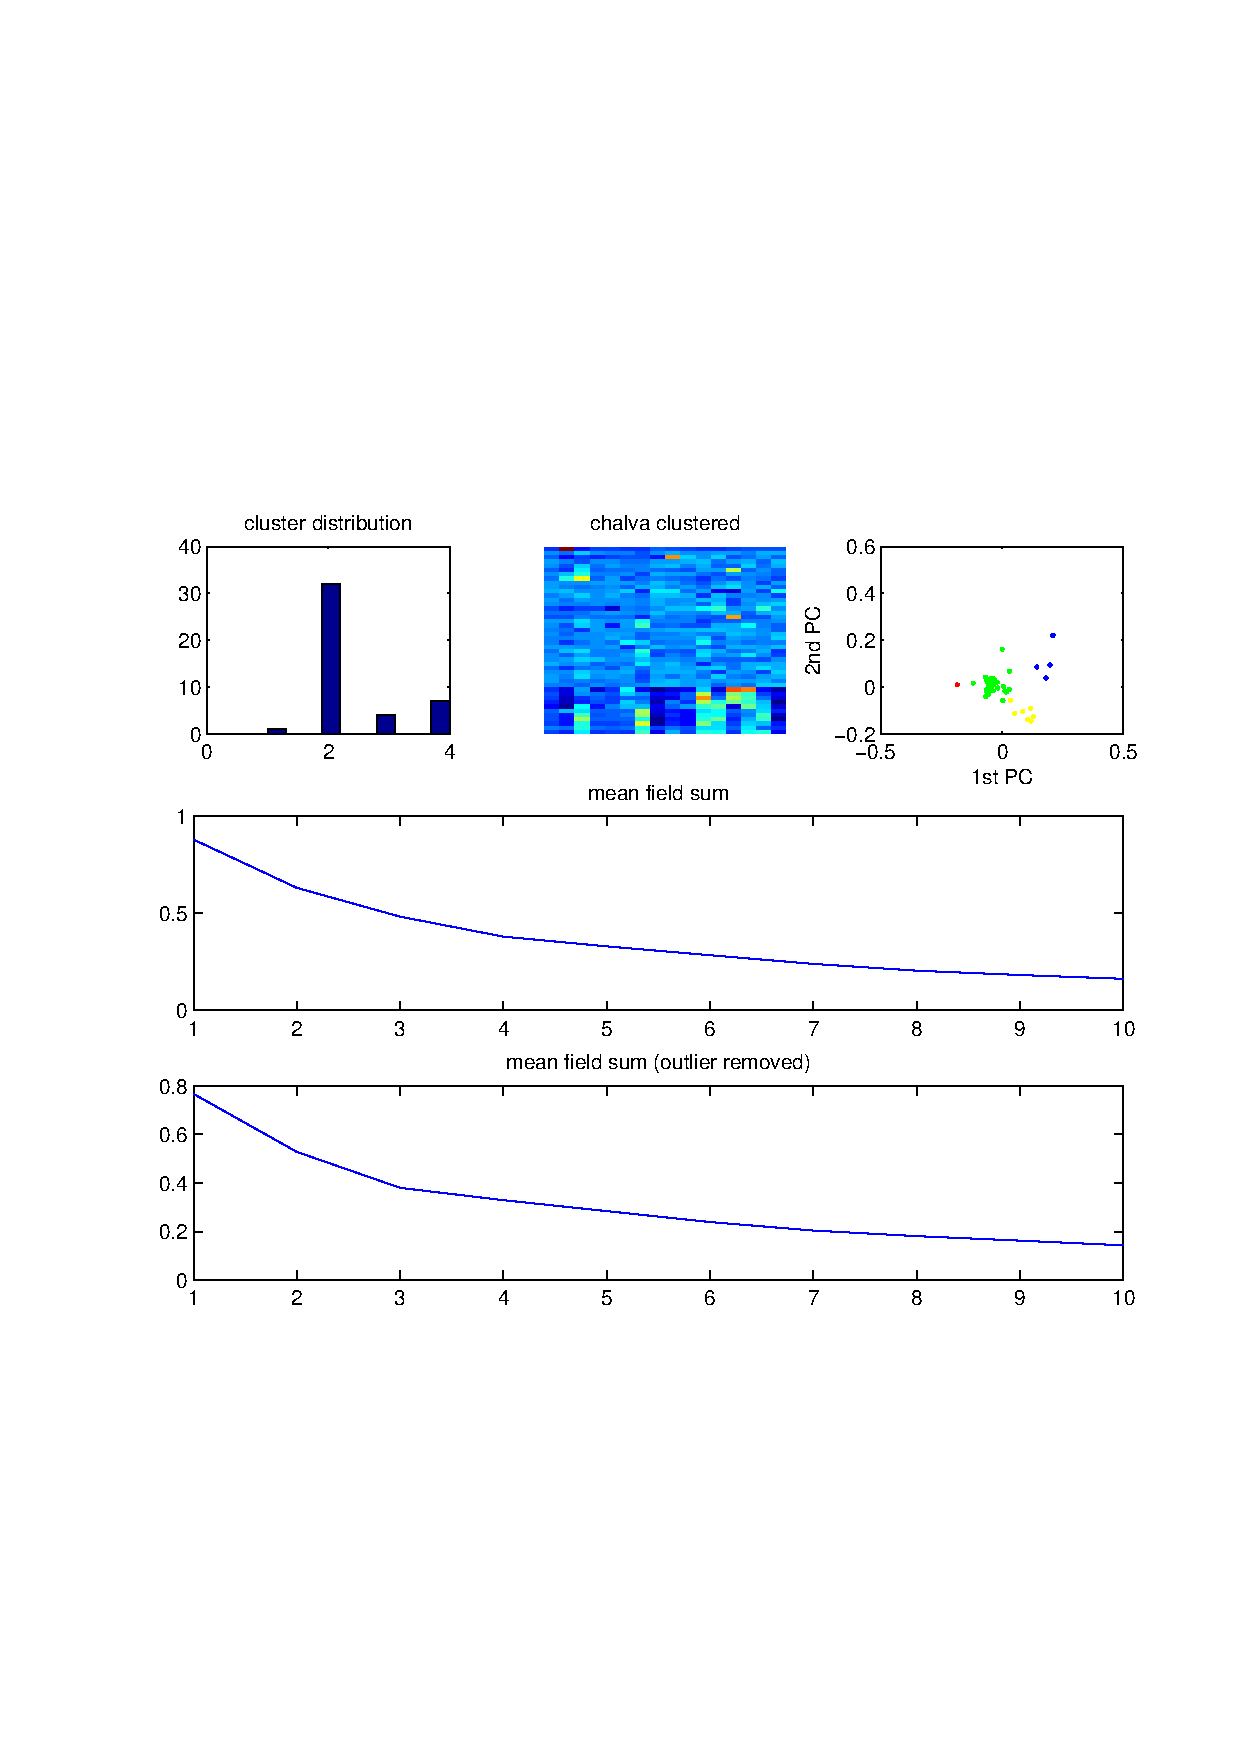
\includegraphics[width=0.8\textwidth]{images/raw_clusters_chalva.pdf}
    \caption{The curve in the middle suggests a clustering with four prototypes, but when such a clustering is done, the distribution of which point is assigned to which cluster (topleft figure) shows that there is an extreme outlier which gets its own cluster. When this outlier is removed from the data, the mean distance plot (lowest plot) shows a clear \emph{elbow} for 3 clusters. The topright plot shows the clusters in the data when projected on their first two principal components.}
    \label{sg:fig:images_raw_clusters_chalva}
\end{figure}
\begin{figure}[ht]
    \centering
        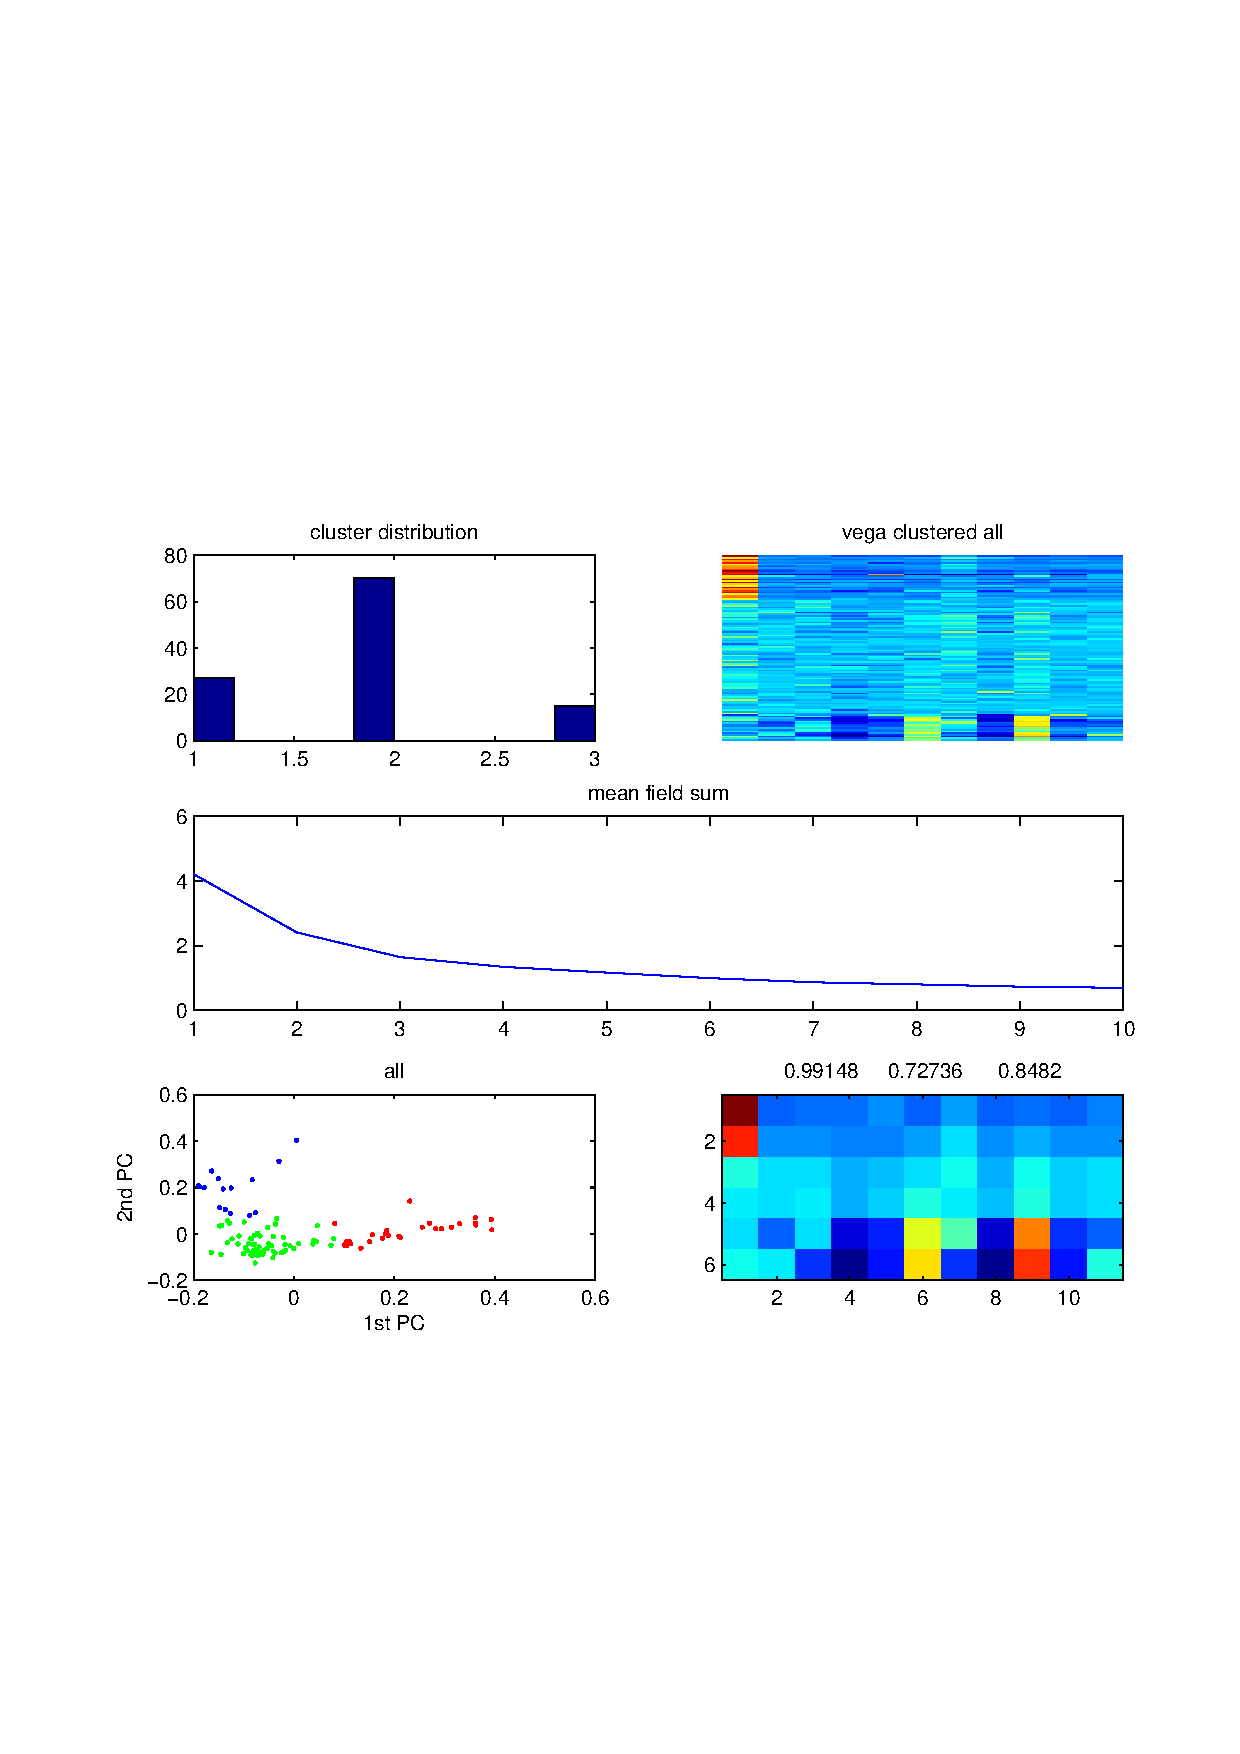
\includegraphics[width=0.8\textwidth]{images/raw_clusters_vega.pdf}
    \caption{For subject V a clearly visible \emph{elbow} (in the center plot) also suggests to cluster the data into three clusters. The topleft plot shows again the distribution of cluster membership and the topright one the clustered data. The lower-left plot is again a projection on the principal components and the lower-right shows similarity of clusters prototypes when the data was first separated by hand-posture. On top of this last plot the matching scores between the clusters are written.}
    \label{sg:fig:Documents_uni_yifat_lab_results_evoked_syns_raw_clusters_vega}
\end{figure}


\begin{figure}[ht]
    \centering
        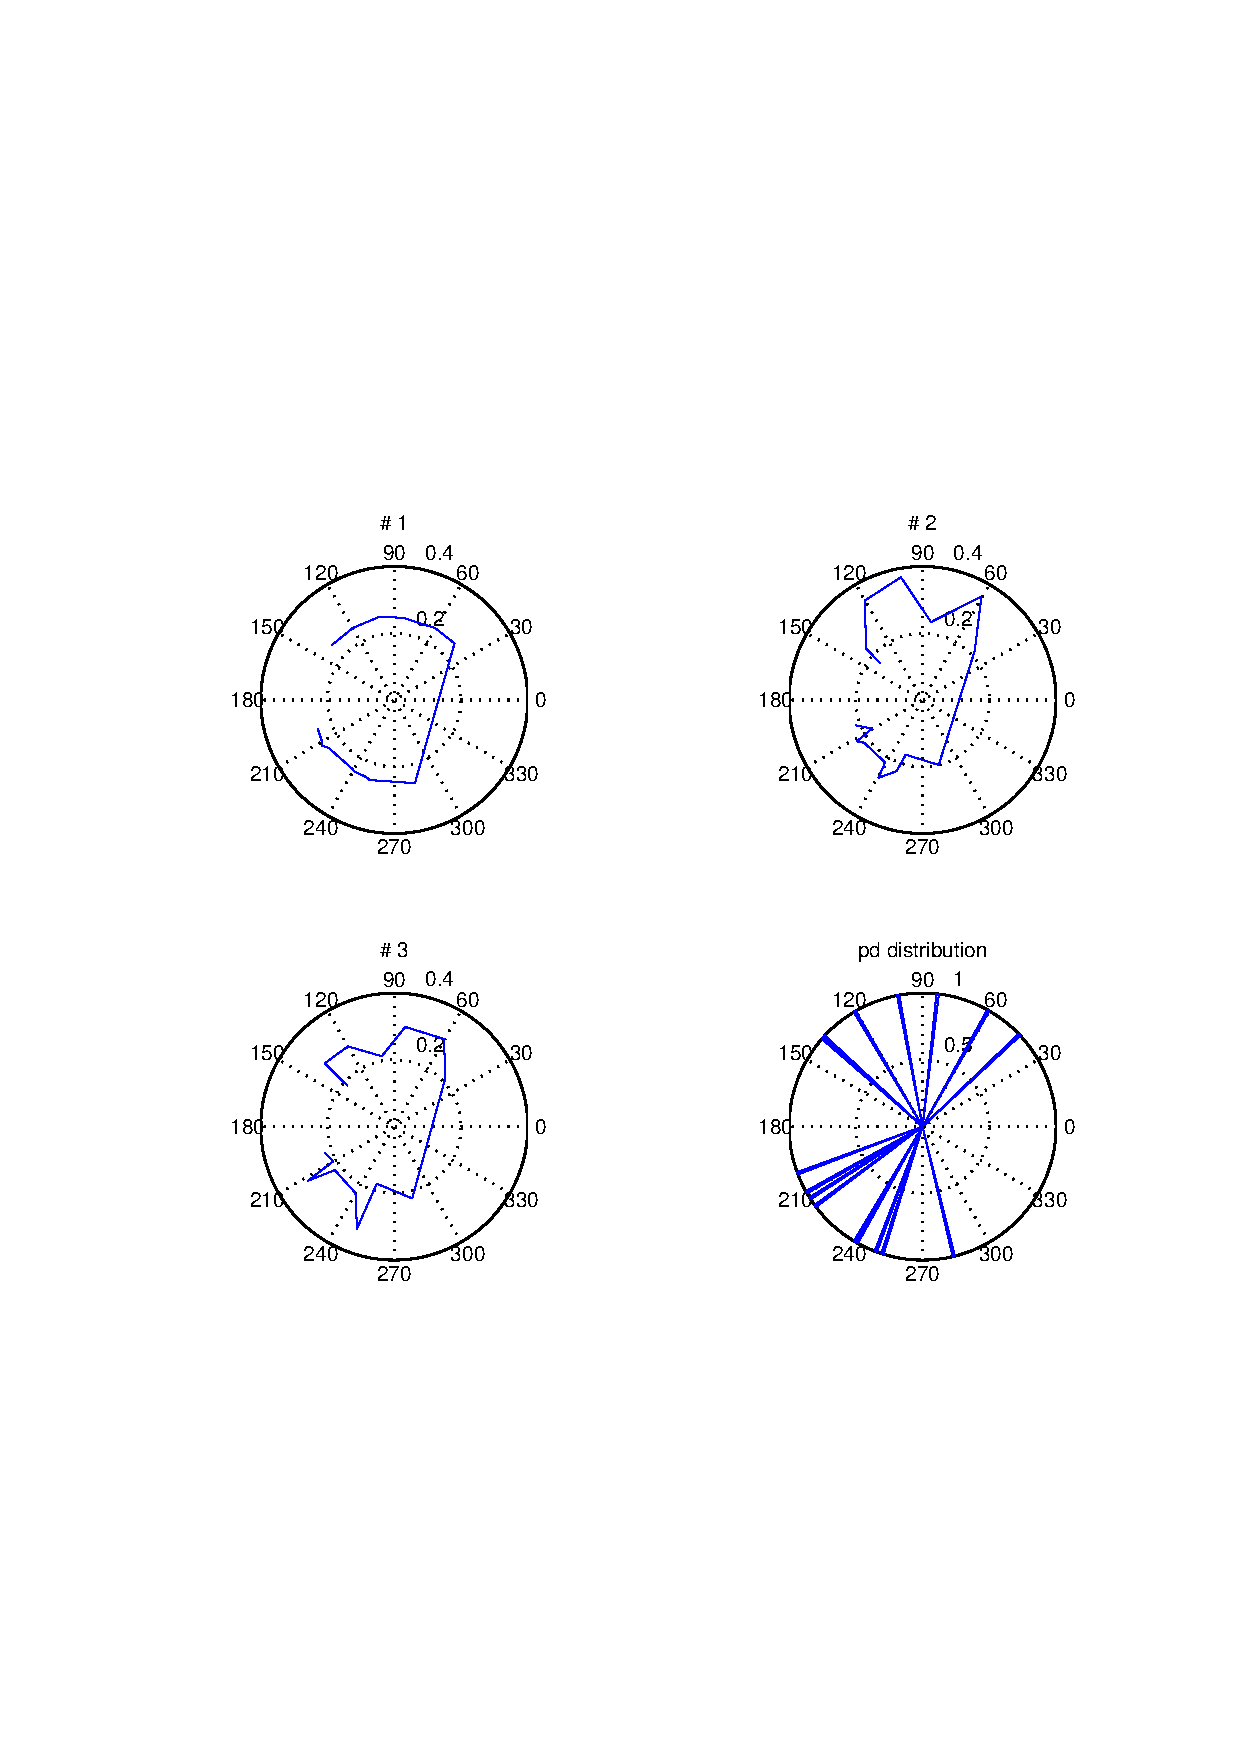
\includegraphics[width=0.8\textwidth]{images/center_rose_chalva.pdf}
    \caption{Clusters of subject C plotted in the PD space. PDs computed during the natural movement. The PDs from the pronation handposition are used for this plot}
    \label{sg:fig:images_center_rose_chalva}
\end{figure}
\begin{figure}[ht]
    \centering
        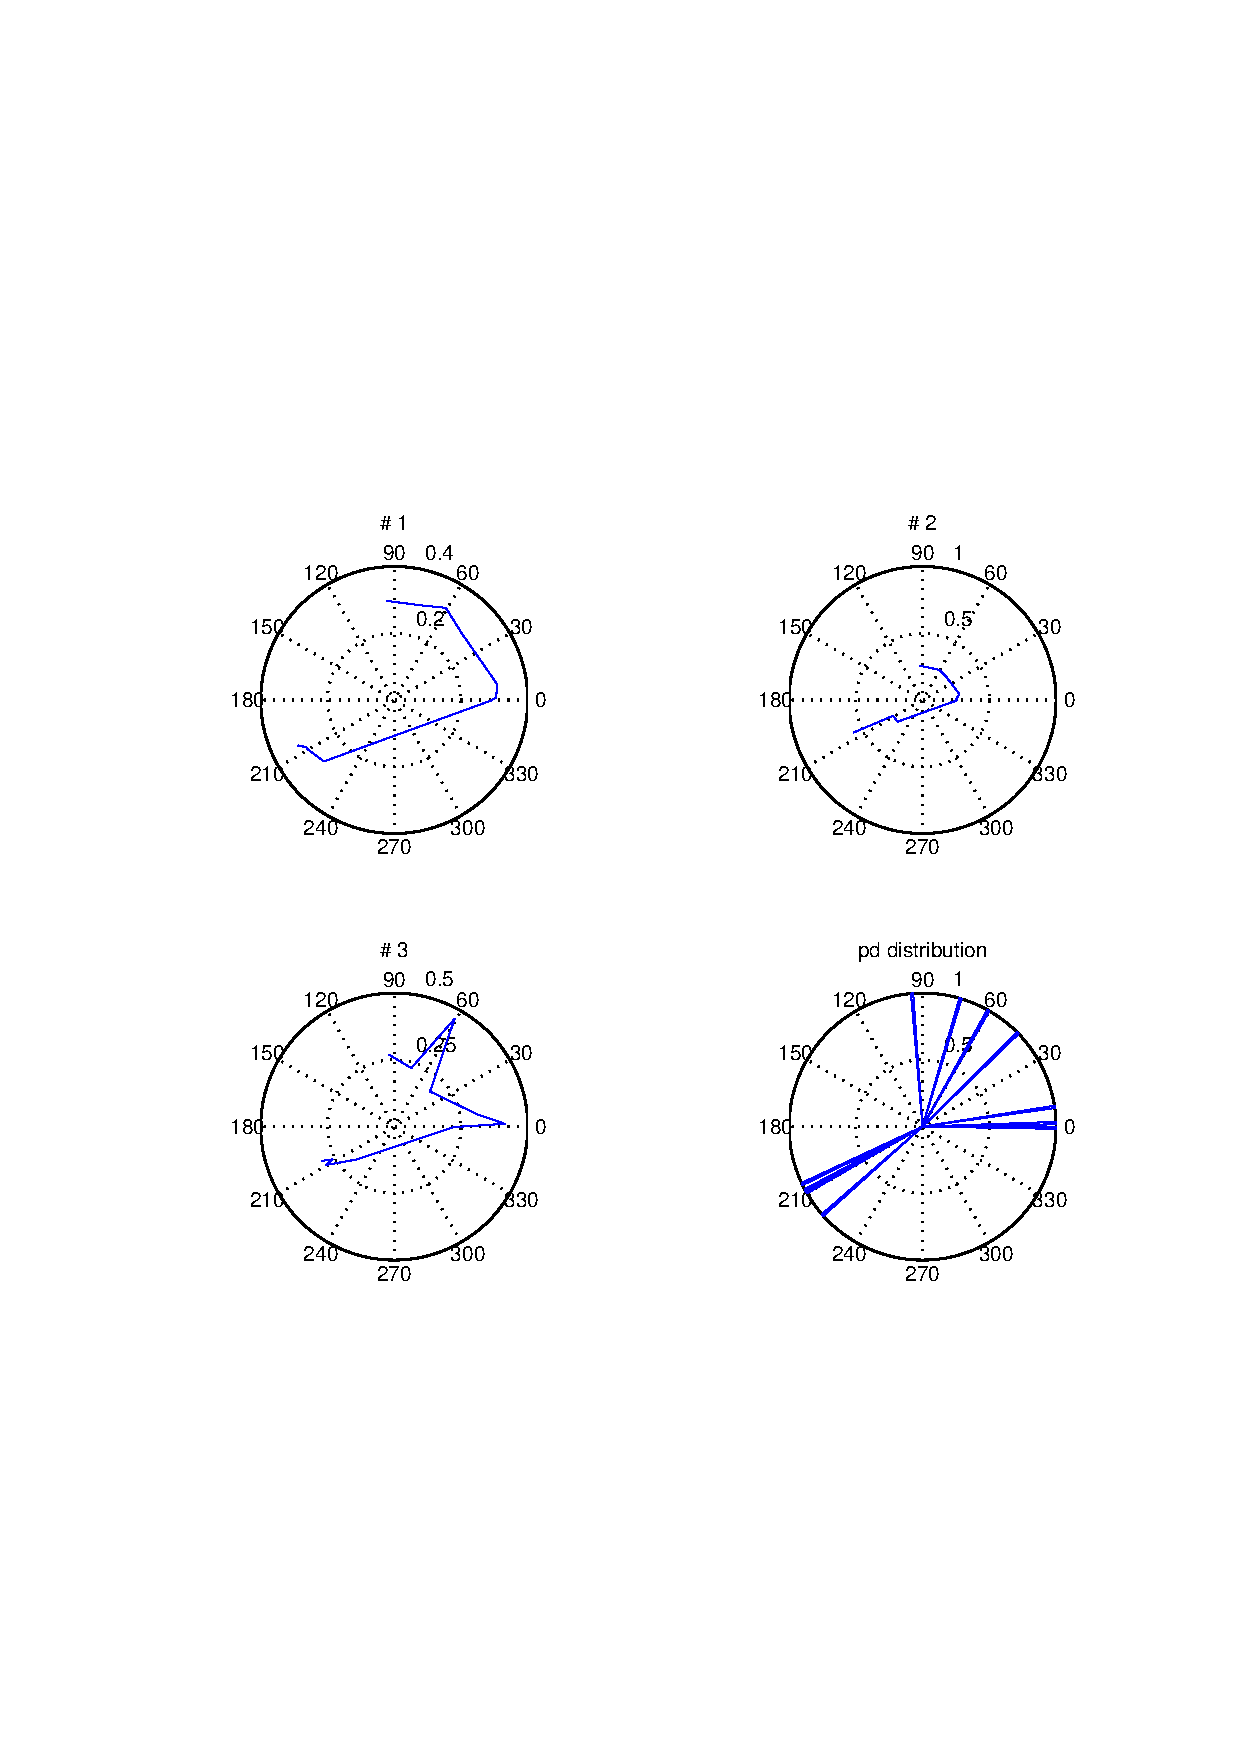
\includegraphics[width=0.8\textwidth]{images/center_rose_vega.pdf}
    \caption{Clusters of subject V plotted in the PD space. PDs computed during the natural movement. The PDs from the pronation handposition are used for this plot}
    \label{sg:fig:images_center_rose_vega}
\end{figure}




Interesting is to plot the cluster membership on the cortex which reveals for both subjects that there is a type of response which can be evoked all over the area in which stimulation took place but there are also responses which are clearly related to the stimulation site. 
\begin{figure}[ht]
    \centering
        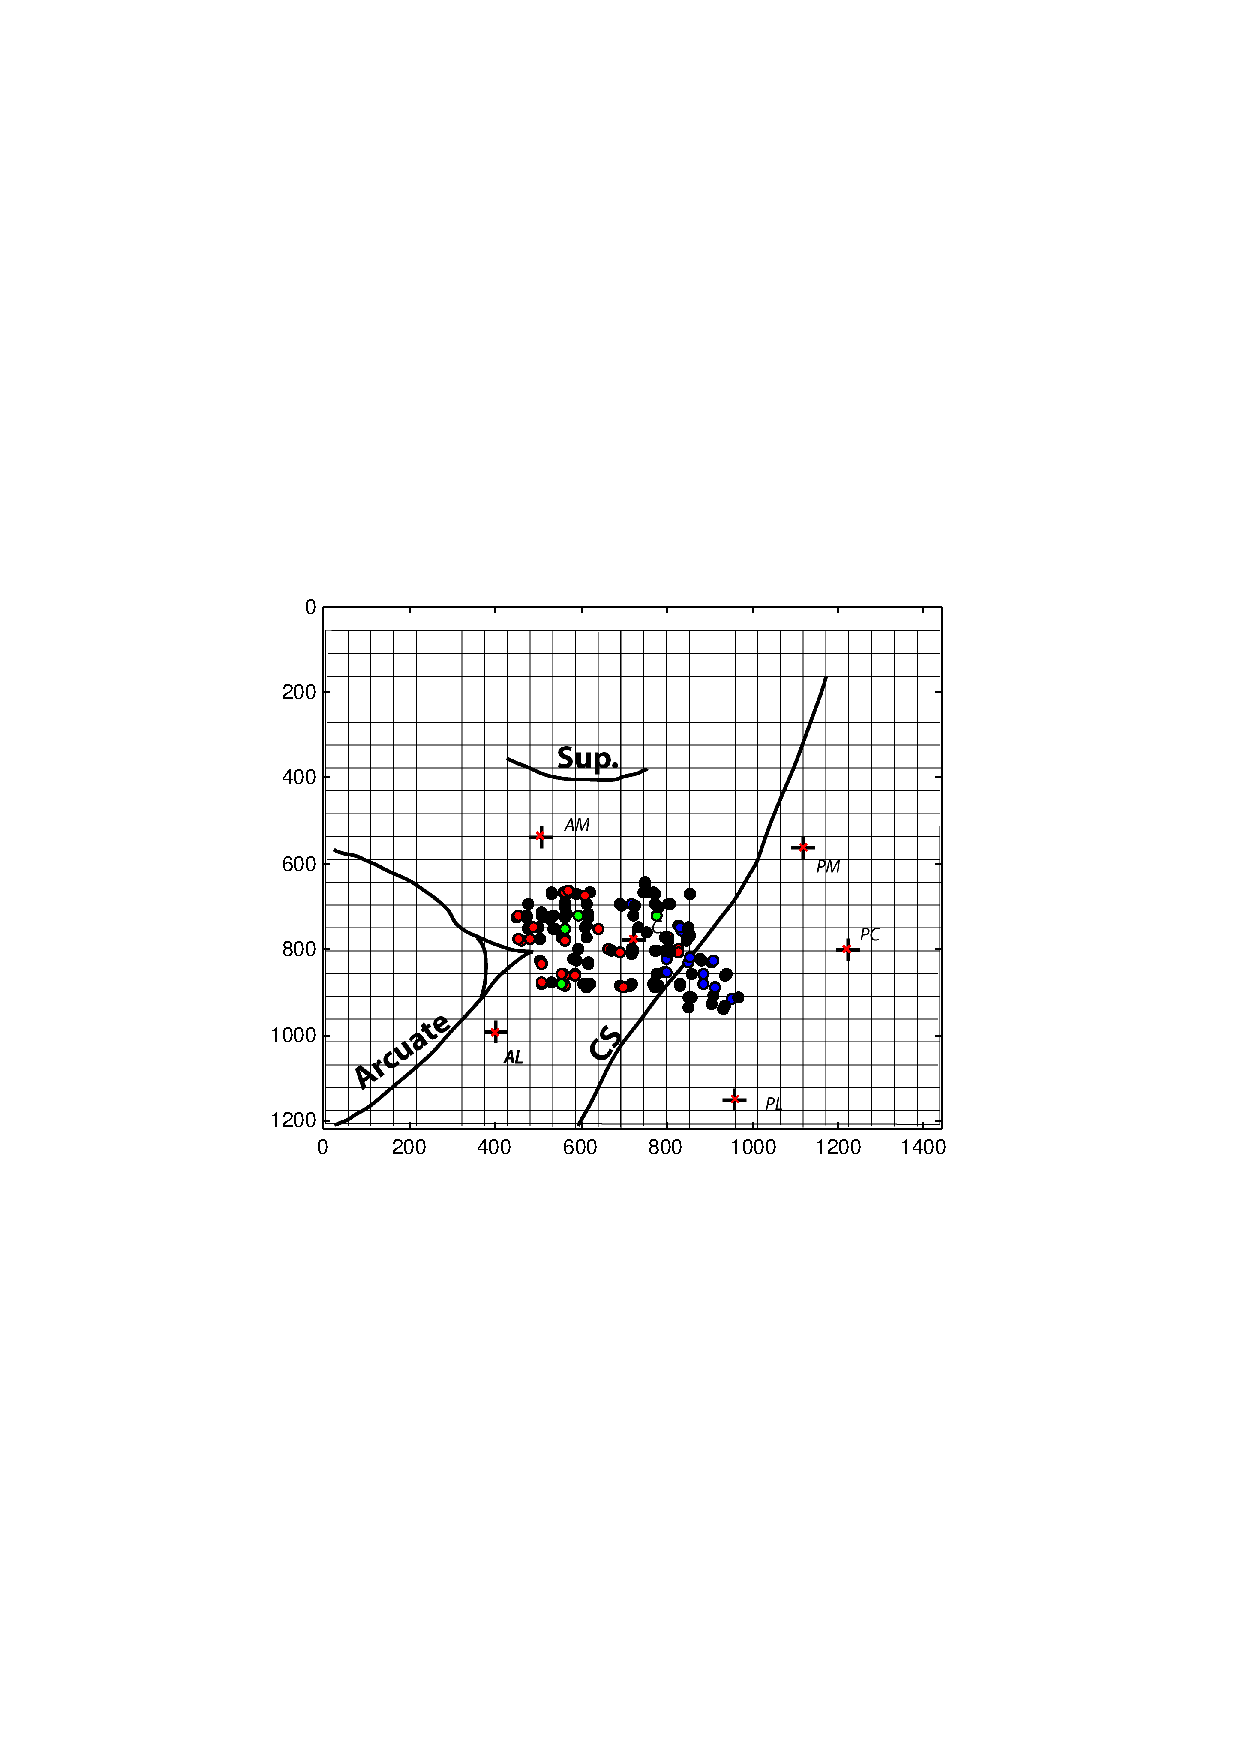
\includegraphics[width=0.8\textwidth]{images/cluster_vega.pdf}
    \caption{clusters on cortex (subject V)}
    \label{sg:fig:images_cluster_vega}
\end{figure}
\begin{figure}[ht]
    \centering
        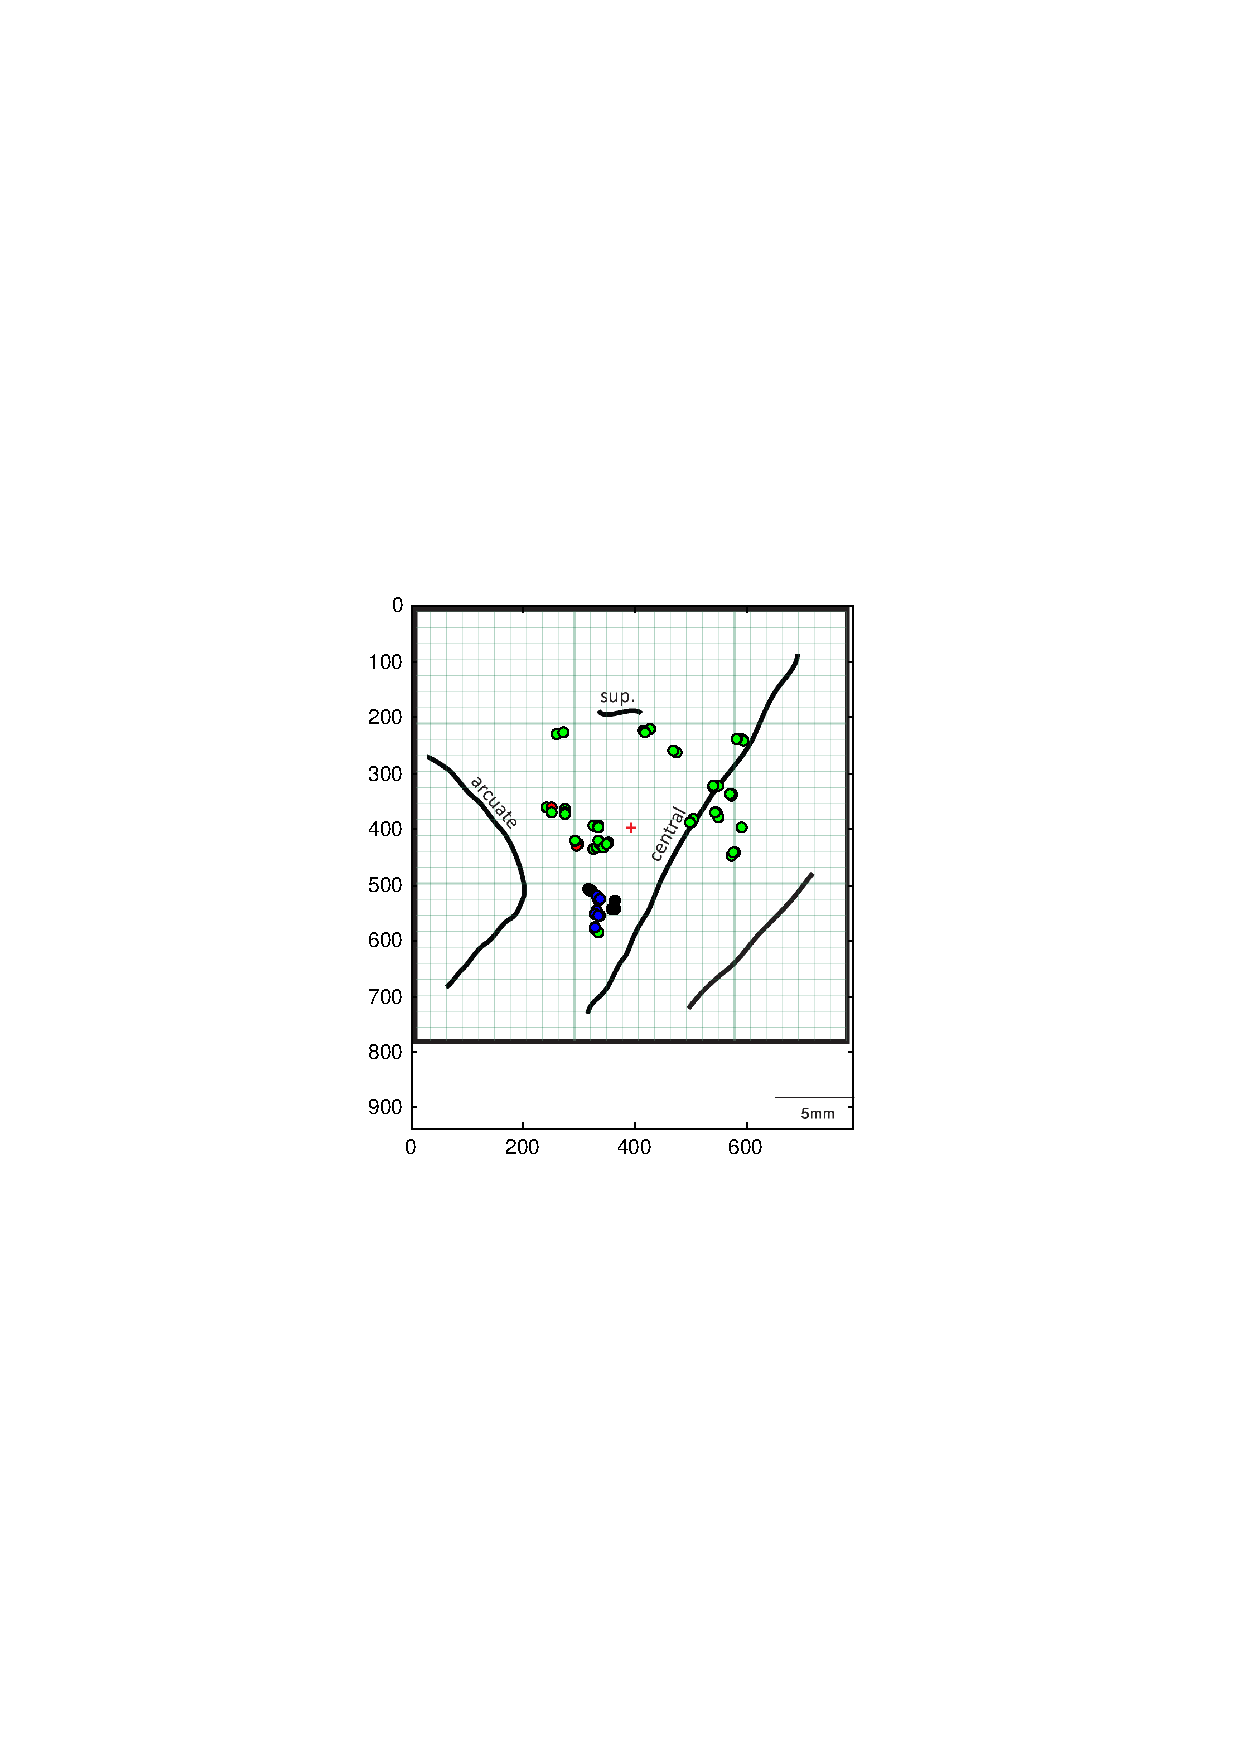
\includegraphics[width=0.8\textwidth]{images/cluster_chalva.pdf}
    \caption{clusters on cortex (subject C)}
    \label{sg:fig:images_cluster_chalva}
\end{figure}


\clearpage

% section evoked_syns (end)




% ============================================================
% = synergy relation, synergies in pd space, projection, etc =
% ============================================================
\section{Relation between evoked activation patterns and natural movement} % (fold)
\label{sg:sec:synergy_relations}

The preferred directions that were computed for each muscle in each recording session showed to be stable over recording days. There is a significant and also visually obvious difference of preferred directions depending on the posture of the hand~\rref{sg:fig:pd_featherplots}. As the PDs showed to be stable over recording sessions, for each muscle the average over sessions was computed and used for further analysis.


\todo{rewrite this paragraph}

The question, whether the cortical stimulation induced responses are just arbitrary activations of muscles that contain some structure but are not related to natural activation patterns or whether they have something in common with the activation patterns that were found during natural movement is an interesting question. If this were the case, it would imply that the stimulation sites are in fact the sites where neuronal activation causes modular organized muscle response patterns, if these happen to be found during natural movement. 

In order to compare the evoked responses with the synergies found during natural movement evaluation of projections onto different subspaces was applied. The natural movement synergies computed on the pooled data from all sessions were used for this method. The data from evoked responses was projected onto the orthonormalized subspace that is spanned by the synergies and also on its orthogonal complement. The ratio of the vector sums of the data projected onto the two subspaces was for the evoked responses significantly higher than for random or randomized data. Although it is not a quantitative measure that gives a value for the relation between the two, the result suggests that there is a significant relation between the muscle response patterns, evoked by cortical stimulation and the synergies extracted from natural movement.


\begin{figure}[ht]
\centering
\subfigure[Subject C]{
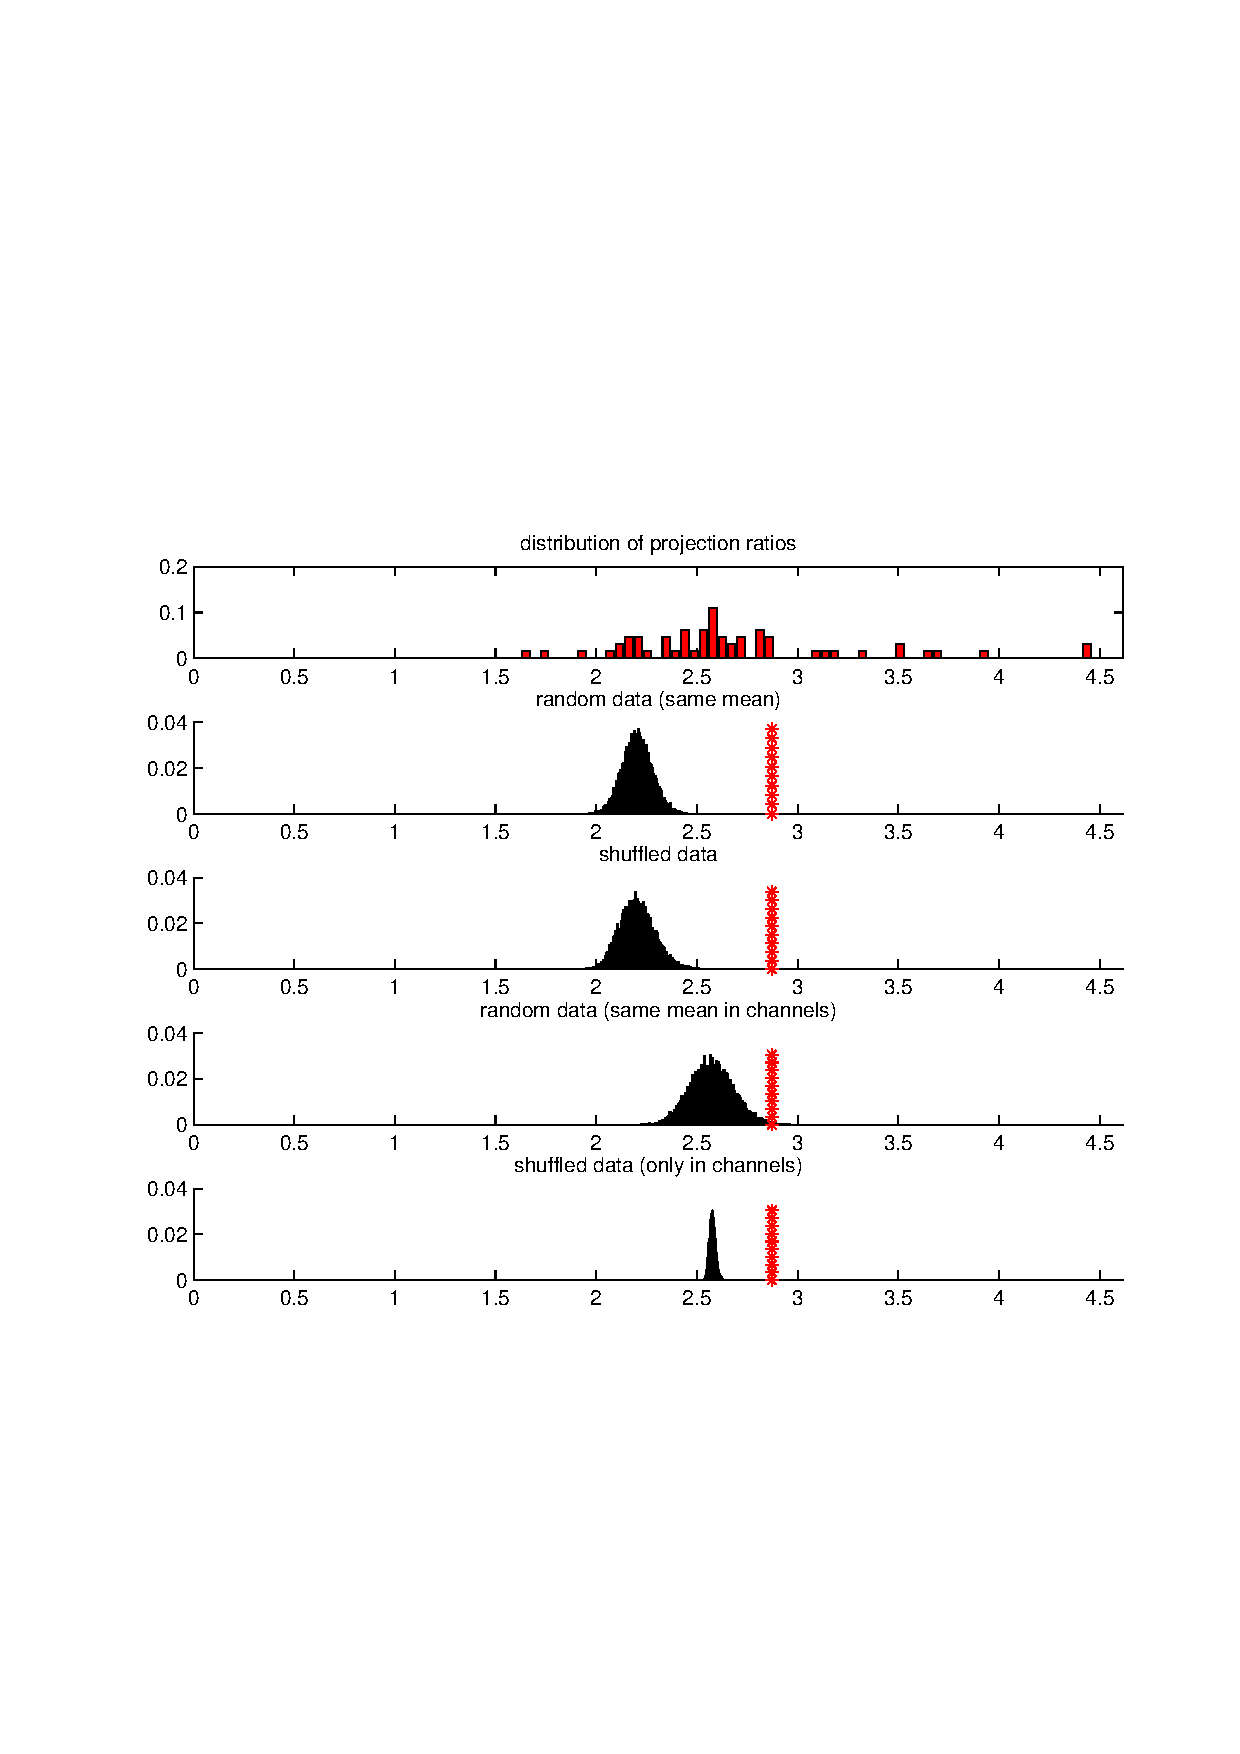
\includegraphics[width=0.4\textwidth]{images/projection_chalva.pdf}
\label{fig:subfig1}
}
\subfigure[Subject V]{
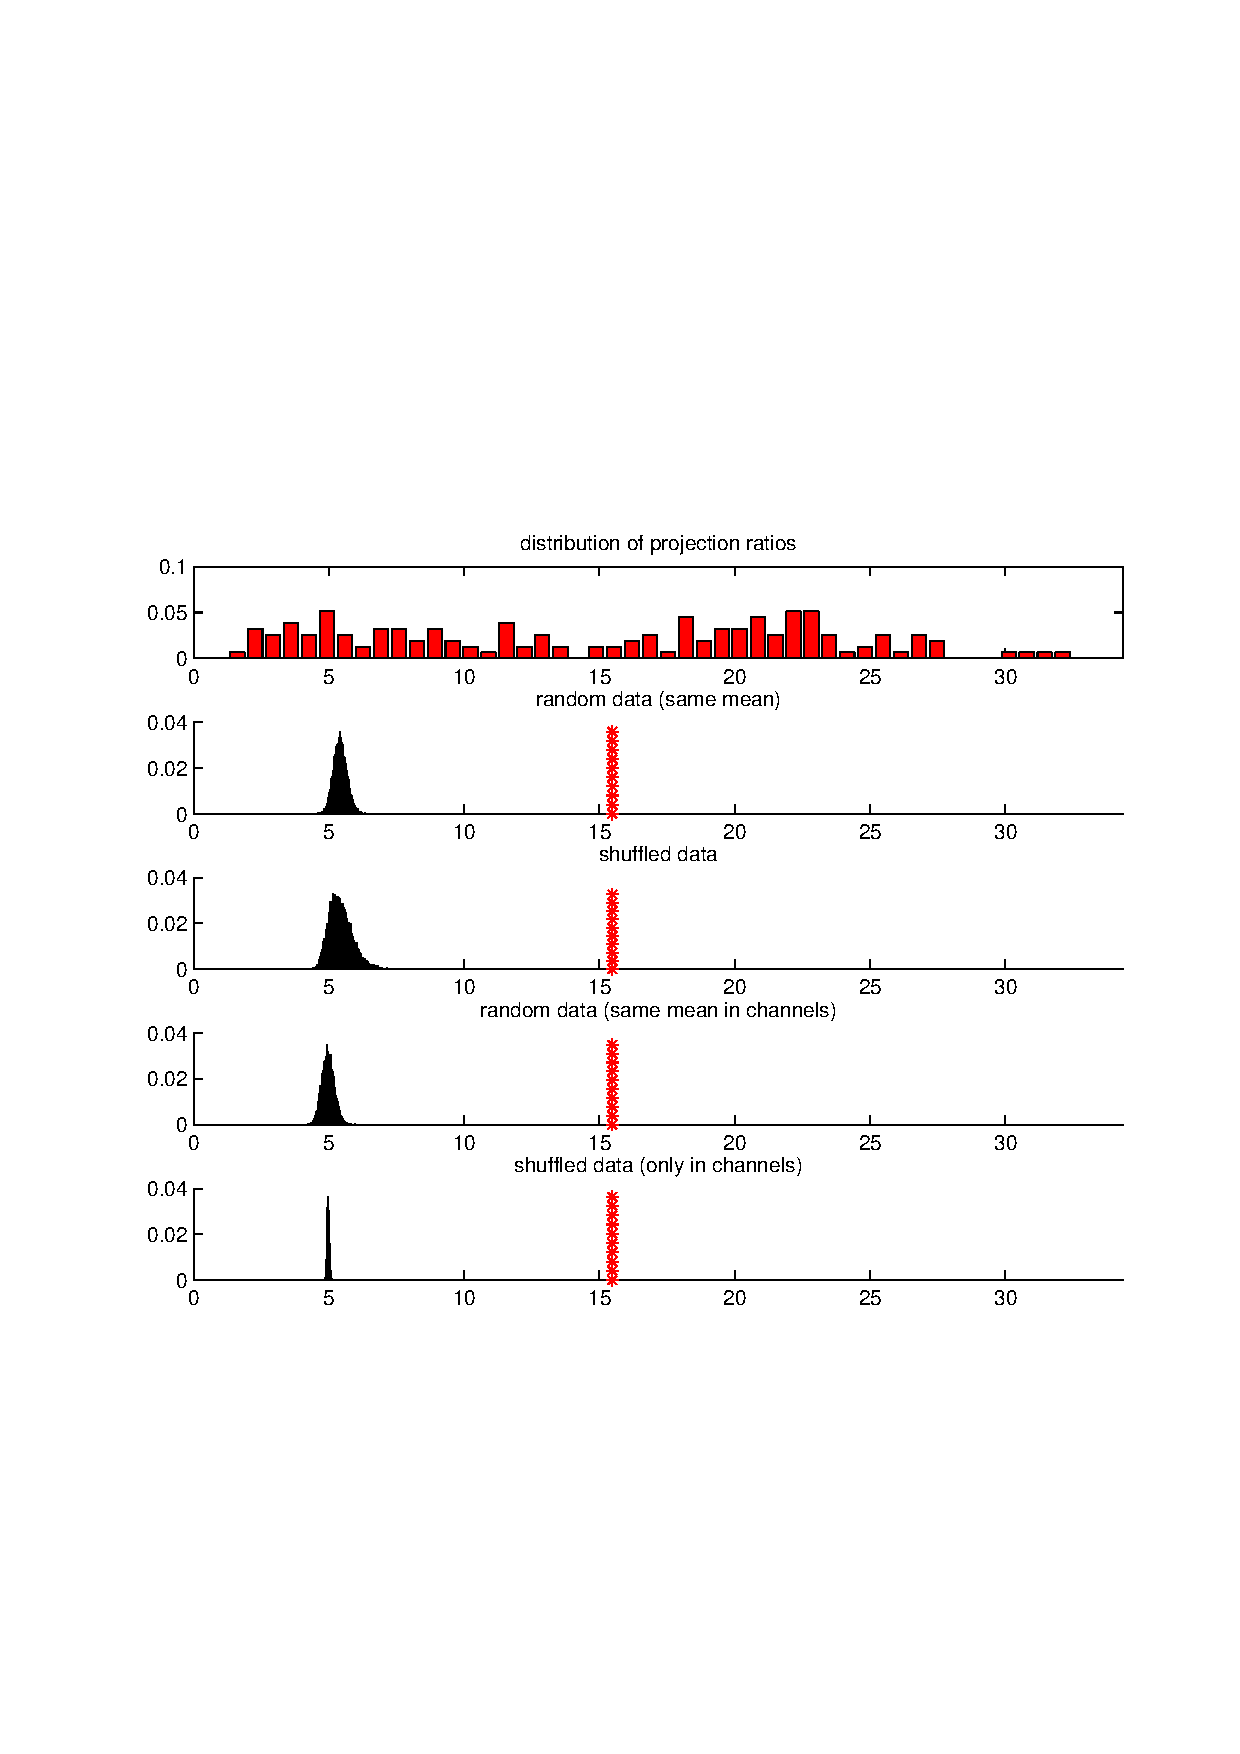
\includegraphics[width=0.4\textwidth]{images/projection_vega.pdf}
\label{fig:subfig2}
}
\caption{Projection ratios of evoked responses, compared to 10000 runs of data with same statistical properties and shuffled versions of itself. The red line is the projection ratio of the original and un-shuffled evoked responses. It clearly shows that the evoked responses reside much more in the subspace spanned by the synergies than random data with same statistical properties.}
\end{figure}



% section synergy_relations (end)




% section results (end)
